% =================================================================
%  NSW Road Crash Analytics — Preliminary Report (INFT6201)
%  Compile: pdflatex -> biber -> pdflatex -> pdflatex  (or latexmk -pdf)
% =================================================================
\documentclass[11pt,a4paper]{article}

% ---------- Packages ----------
\usepackage[T1]{fontenc}
\usepackage[utf8]{inputenc}
\usepackage{lmodern}
\usepackage{microtype}
\usepackage[a4paper,margin=2.5cm]{geometry}
\usepackage{amsmath,amssymb}
\usepackage{graphicx}
\usepackage{listings}
\usepackage{booktabs}
\usepackage{tabularx}
\usepackage{longtable}
\usepackage{array}
\usepackage{float}
\usepackage[font=small,labelfont=bf]{caption}
\usepackage{enumitem}
\usepackage{xcolor}
\usepackage{tikz}
\usetikzlibrary{positioning,shapes.multipart,decorations.pathreplacing}
\usepackage{fancyhdr}
\usepackage{titlesec}
\usepackage[english]{babel}
\usepackage{csquotes}
\usepackage[style=apa,backend=biber]{biblatex}
\addbibresource{references.bib}
\usepackage[hidelinks]{hyperref}

\graphicspath{{../figures/}}

\lstset{language=Python, basicstyle=\ttfamily\scriptsize, numbers=left, numberstyle=\tiny\color{gray},
        numbersep=6pt, breaklines=true, breakatwhitespace=false, columns=fullflexible, keepspaces=true,
        frame=single, rulecolor=\color{gray!40}, backgroundcolor=\color{gray!4},
        keywordstyle=\color{accent}\bfseries, commentstyle=\color{gray}\itshape, stringstyle=\color{orange!70!black},
        showstringspaces=false, captionpos=t, xleftmargin=1.5em, framexleftmargin=1.5em,
        literate={–}{{--}}1 {—}{{---}}1 {×}{{$\times$}}1 {≤}{{$\le$}}1}

% ---------- Styling ----------
\definecolor{accent}{HTML}{1C5CAB}
\titleformat{\section}{\Large\bfseries\color{accent}}{\thesection}{0.8em}{}
\titleformat{\subsection}{\large\bfseries}{\thesubsection}{0.8em}{}
\setlength{\parskip}{0.5em}
\setlength{\parindent}{0pt}
\setlist{itemsep=0.2em,topsep=0.3em}
\newcolumntype{L}{>{\raggedright\arraybackslash}X}
\newcolumntype{P}[1]{>{\raggedright\arraybackslash}p{#1}}
\newcolumntype{R}{>{\raggedleft\arraybackslash}X}

\pagestyle{fancy}
\fancyhf{}
\lhead{\small NSW Road Crash Analytics}
\rhead{\small INFT6201 Project Report}
\cfoot{\small\thepage}
\renewcommand{\headrulewidth}{0.4pt}

% =================================================================
\begin{document}

% ---------- Title page ----------
\begin{titlepage}
  \centering
  \vspace*{3cm}
  {\Large\color{accent} INFT6201 --- Data Science Project\par}
  \vspace{1.2cm}
  {\Huge\bfseries Who Gets Hurt, Where and Why?\par}
  \vspace{0.4cm}
  {\Large Severity analytics on New South Wales road crash data, 2020--2024\par}
  \vspace{2cm}
  {\large Quang Thanh Dong\par}
  {\large Student ID: [your student number]\par}
  \vspace{0.6cm}
  {\large Master of Information Technology, Trimester 3, 2026\par}
  \vfill
  {\small Code and reproducible outputs: \url{https://github.com/QuangThanhDS/nsw-road-crash-analytics}\par}
  \vspace{0.5cm}
  {\small \today\par}
\end{titlepage}

% ---------- Executive summary ----------
\section*{Executive summary}
\addcontentsline{toc}{section}{Executive summary}

New South Wales (NSW) recorded 340 road deaths in 2024, and the State's 2026 Road Safety Action Plan
commits to halving deaths and cutting serious injuries by 30\% by 2030
\parencite{tfnsw_actionplan,tfnsw_toll2024}. This report uses the Transport for NSW open crash data
for 2020--2024 \parencite{tfnsw_crashdata}, which covers 92,082 police-reported crashes and 1,507 deaths, to ask
which crash circumstances turn a crash into a fatal or serious one, and where those crashes happen.

Three findings stand out from the preliminary analysis:
\begin{itemize}
  \item \textbf{Regional rural roads carry a disproportionate share of trauma.} They account for 12.7\% of
        crashes but 39.2\% of deaths. At the same posted speed limit, a crash outside Greater
        Sydney--Newcastle--Wollongong is roughly two to four times more likely to be fatal (5.0\% vs 1.4\% at 100\,km/h).
  \item \textbf{Who is involved matters more than when or in what weather.} Crashes involving a motorcycle,
        pedestrian or cyclist, or a collision with a tree or pole, carry the highest odds of a killed or
        seriously injured (KSI) outcome. Weather and day of week add almost nothing.
  \item \textbf{Data quality can mislead a model.} The \emph{Street lighting} field is left
        \enquote{unknown} far more often for minor crashes than for fatal ones, which leaks the outcome into the
        model. Removing it lowers the apparent ROC-AUC from 0.81 to a more honest 0.75.
\end{itemize}

A temporally validated gradient-boosting model ranks 2024 crashes well (the top risk decile has a 61\% KSI
rate against 5.5\% in the bottom decile), and an interpretable logistic regression performs almost as well.
That makes logistic regression the better fit for public-sector stakeholders who need to explain their
decisions.

\tableofcontents
\newpage

% =================================================================
\section{Case study}
\label{sec:case}

\subsection{Context}
Road trauma is a leading cause of preventable death worldwide \parencite{who_2023}. In NSW, more than two-thirds
of road deaths occur on country roads, even though country residents make up about one-third of the
population \parencite{tfnsw_actionplan}. The 2026 Road Safety Action Plan sets targets of a 50\% reduction in
deaths and a 30\% reduction in serious injuries from the 2018--2020 baseline by 2030 \parencite{tfnsw_actionplan}.
Meeting these targets needs evidence on \emph{which} crashes become severe, so that limited
infrastructure, enforcement and education budgets can go where they prevent the most trauma.

\subsection{Application examples}
The analysis is designed to support decisions such as:
\begin{itemize}
  \item \textbf{Safer-roads investment:} prioritising route segments with clusters of severe run-off-road and
        head-on crashes for barriers, rumble strips or tree and pole treatments.
  \item \textbf{Vulnerable road user programs:} targeting motorcycle, pedestrian and cyclist safety where
        these users make up a large share of KSI crashes.
  \item \textbf{Enforcement and patrol scheduling:} aligning police resources with the times and places where
        crashes are most likely to be severe, not just most frequent.
  \item \textbf{Speed-zone review:} using severity differences across speed limits and regions to inform
        reviews of 80--110\,km/h rural zones.
\end{itemize}

\subsection{Data science questions}
\begin{enumerate}[label=\textbf{Q\arabic*.}]
  \item \textbf{Severity factors:} Which road, environment and road-user characteristics are associated with a
        reported crash being fatal or serious (KSI), and how well can they predict it?
  \item \textbf{Regional gap:} Why are regional crashes more severe than metropolitan ones, and does the gap
        persist after accounting for speed limit and crash type?
  \item \textbf{Hotspots:} Where are crashes and severe crashes concentrated, and which local government areas
        (LGAs) carry the largest burden?
  \item \textbf{Temporal patterns:} How do volume and severity vary by year (including the COVID-19 period),
        day of week and time of day?
\end{enumerate}
This preliminary report answers Q1 with initial models and gives descriptive evidence for Q2--Q4.

\subsection{Stakeholders}
Table~\ref{tab:stakeholders} lists the main stakeholders and how each would use the results.

\begin{table}[H]
\centering
\caption{Key stakeholders and their interest in the analysis.}
\label{tab:stakeholders}
\small
\begin{tabularx}{\textwidth}{@{}P{4.2cm}L@{}}
\toprule
\textbf{Stakeholder} & \textbf{Interest and use of results} \\
\midrule
Transport for NSW, Centre for Road Safety & Data custodian and policy owner; program targeting, progress against 2030 targets \\
Local councils & Local road treatments, 40\,km/h zones, LGA-level benchmarking \\
NSW Police Force & Timing and location of enforcement (e.g.\ weekend mornings, regional highways) \\
NSW Health and emergency services & Regional trauma response times and hospital demand \\
Insurers (icare, CTP insurers) & Injury burden and claims risk \\
Road user advocacy groups & Evidence for motorcycle, cycling and pedestrian safety \\
General public & Transparent communication of risk \\
\bottomrule
\end{tabularx}
\end{table}

% =================================================================
\section{Datasets}
\label{sec:data}

\subsection{Background}
The primary source is the \emph{NSW Road Crash Data 2020--2024} release published by Transport for NSW on its
Open Data Hub under a Creative Commons Attribution licence \parencite{tfnsw_crashdata}. The release is
updated annually as a rolling five-year window; the 2020--2024 release (updated 9 October 2025) is the
most recent available. It contains crashes that meet national reporting criteria: the crash was reported to
police, occurred on a public road, involved at least one moving vehicle, and resulted in a death, an injury
or a vehicle being towed away \parencite{tfnsw_manual}.

The data comes as two linked tables (Table~\ref{tab:datasets}). The \emph{Data Manual} defines every field
\parencite{tfnsw_manual}. Severity levels below \enquote{fatal} come from linking police reports with health
records: a \emph{serious injury} crash is one where at least one person was matched to a hospital admission on
the day of the crash or the day after, while a \emph{moderate injury} is matched only to an emergency department
attendance. Fatalities are deaths within 30 days of the crash.

To map the data, simplified Australian Statistical Geography Standard (ASGS) Edition 3 boundaries for the
state, Greater Sydney and 2024 LGAs were used \parencite{abs_asgs}. They were obtained in converted form
from the \texttt{nswgeo} package \parencite{suster_nswgeo}.

\begin{table}[H]
\centering
\caption{Datasets used in the analysis.}
\label{tab:datasets}
\small
\begin{tabularx}{\textwidth}{@{}P{3.4cm}P{2.3cm}L@{}}
\toprule
\textbf{Table} & \textbf{Size} & \textbf{Content} \\
\midrule
CRASH & 92,189 rows $\times$ 50 columns & One row per crash: year, month, weekday, two-hour time band, location (coordinates,
LGA, suburb, street), road and environment (speed limit, alignment, surface, weather, lighting), crash type
(RUM/DCA codes, first impact type), key vehicle type, and counts of people killed and injured by severity. \\
TRAFFIC UNIT & 170,962 rows $\times$ 10 columns & One row per traffic unit (vehicle, pedestrian, cyclist): unit type, role in first impact,
direction, manoeuvre and objects hit. Linked to CRASH by \texttt{Crash ID} (one-to-many). \\
ASGS boundaries & 1 state, 1 GCCSA, 129 LGAs & Polygon boundaries (GDA2020) used for mapping. \\
\bottomrule
\end{tabularx}
\end{table}

\subsection{Data quality issues}
A systematic profile of all 50 CRASH fields (missing values, \enquote{unknown}-coded values, cardinality and
range checks) and a referential-integrity check between tables found the issues summarised in
Table~\ref{tab:dq}. The structure of the data is clean: there are no duplicate crash IDs and no orphan traffic
units, and every crash has at least one unit. The problems lie in \emph{what was recorded and how}.

\begin{table}[H]
\centering
\caption{Data quality issues identified and how they were handled.}
\label{tab:dq}
\small
\begin{tabularx}{\textwidth}{@{}P{3.2cm}LP{4.2cm}@{}}
\toprule
\textbf{Issue} & \textbf{Evidence} & \textbf{Handling} \\
\midrule
Outcome-dependent recording (target leakage) &
\emph{Street lighting} is \enquote{Unknown / not stated} for 36.5\% of crashes overall, but for 62.8\% of
tow-away and 52.9\% of minor-injury crashes compared with 0.6\% of fatal ones. The KSI rate is 3.6\% when the field
is unknown and 26--38\% otherwise. &
Excluded from the main model; a comparison run quantifies the leakage (Section~\ref{sec:prelim}). \\
\addlinespace
Structural missingness &
\emph{Primary temporary / hazardous / permanent feature} are 98.5\%, 98.0\% and 73.0\% blank; \emph{Other TU type}
is 30.4\% blank (single-vehicle crashes). A blank means \enquote{none}, not \enquote{unknown}. &
Not used yet; to be recoded as \enquote{None}. \\
\addlinespace
Coverage and under-reporting &
Only police-reported injury or tow-away crashes are included; minor crashes without a tow-away are absent. &
Results describe severity \emph{given} a reported crash, not crash risk per trip. \\
\addlinespace
Late reporting &
107 crashes from 2019 appear in reporting year 2020, and 63--167 crashes each year are reported in the
following year. &
Analysis uses \emph{Year of crash} and keeps 2020--2024 only (92,082 crashes). \\
\addlinespace
Consistency with official totals &
Deaths in the data match the official 2023 toll (340) exactly, but 2024 shows 327 against an official 340
\parencite{tfnsw_toll2024}. &
Noted; 2024 counts may be revised in later releases. \\
\addlinespace
Definitional overlap &
\emph{Urbanisation} is itself derived from LGA and speed limit (country urban $\leq$80\,km/h, non-urban
$>$80\,km/h; \cite{tfnsw_manual}). &
Regions are compared as metro vs rest of NSW \emph{within} speed limits. \\
\addlinespace
Coarse time and privacy limits &
Time is given only as two-hour bands, month and weekday. No driver age, licence, speeding, alcohol or
restraint fields are released. &
Time treated as categorical; human factors listed as a limitation. \\
\addlinespace
Spatial outliers &
Five crashes at 159\textdegree E look anomalous but are on Lord Howe Island (part of NSW). &
Kept; excluded only from the mainland map. \\
\bottomrule
\end{tabularx}
\end{table}

The first issue is the most consequential. Police record crash circumstances in more detail when someone is
badly hurt. As a result, whether a field was \emph{filled in} carries information about the outcome, which is
a classic form of leakage \parencite{kaufman2012}. Smaller \enquote{unknown} categories in \emph{Natural lighting}
and \emph{Key TU type} (each under 2.5\% of crashes) show the same pattern and are flagged for treatment in
the next stage.

% =================================================================
\section{Data modelling}
\label{sec:model}

\subsection{Conceptual data model}
The two source tables form a one-to-many relational model (Figure~\ref{fig:erd}). For analysis, the
TRAFFIC UNIT table was aggregated to the crash level as binary flags (for example \emph{any pedestrian
involved}, \emph{any motorcycle involved}, \emph{tree or pole hit}) and joined to CRASH. This gives one row per
crash, which matches the unit of the severity outcome.

\begin{figure}[H]
\centering
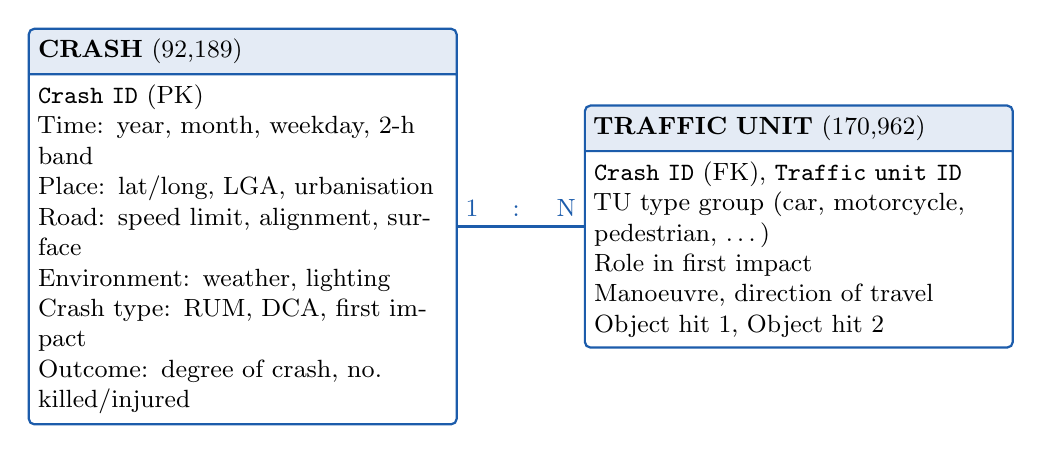
\begin{tikzpicture}[
  entity/.style={rectangle split, rectangle split parts=2, draw=accent, thick, rounded corners=2pt,
                 text width=5.2cm, font=\small, align=left, rectangle split part fill={accent!12,white}},
  node distance=1.6cm]
  \node[entity] (crash) {\textbf{CRASH} (92,189)
    \nodepart{second}\texttt{Crash ID} (PK)\\
    Time: year, month, weekday, 2-h band\\
    Place: lat/long, LGA, urbanisation\\
    Road: speed limit, alignment, surface\\
    Environment: weather, lighting\\
    Crash type: RUM, DCA, first impact\\
    Outcome: degree of crash, no.\ killed/injured};
  \node[entity, right=of crash] (tu) {\textbf{TRAFFIC UNIT} (170,962)
    \nodepart{second}\texttt{Crash ID} (FK), \texttt{Traffic unit ID}\\
    TU type group (car, motorcycle, pedestrian, \ldots)\\
    Role in first impact\\
    Manoeuvre, direction of travel\\
    Object hit 1, Object hit 2};
  \draw[thick, accent] (crash.east) -- node[above, font=\small]{1 \quad : \quad N} (tu.west);
\end{tikzpicture}
\caption{Relational model of the TfNSW crash data. Traffic units are aggregated to crash-level flags before modelling.}
\label{fig:erd}
\end{figure}

\subsection{Analytical problem formulation}
\label{sec:formulation}

\textbf{Unit of analysis.} Each observation is one police-reported crash (92,082 crashes from 2020 to 2024).
The model asks: \emph{given that a crash has happened and been reported, how likely is it that someone was
killed or seriously injured?} It does not predict whether a crash will happen, because the data contains no
exposure measure such as traffic volume or kilometres travelled.

\textbf{What is predicted (target).} Crash severity is an ordered, five-level outcome, but its extremes are very
unbalanced (1.5\% fatal against 32.0\% non-casualty). The preliminary model therefore predicts a binary target
that matches the policy target in the Road Safety Action Plan \parencite{tfnsw_actionplan}:
\begin{equation}
  y_i = \text{KSI}_i =
  \begin{cases}
    1 & \text{if \emph{Degree of crash -- detailed}} \in \{\text{Fatal},\ \text{Serious Injury}\}\\
    0 & \text{if Moderate Injury, Minor/Other Injury or Non-casualty (tow-away)}
  \end{cases}
  \label{eq:target}
\end{equation}
Overall, 22.8\% of crashes are KSI (22.2\% in the training years and 25.1\% in the 2024 test year). The model
outputs a probability $\hat{p}_i = P(y_i = 1 \mid \mathbf{x}_i)$, which is turned into a \enquote{high-risk / not
high-risk} label with a threshold (Section~\ref{sec:validation}). The target is computed in
\texttt{clean\_crash()} (Listing~\ref{lst:features}, line 23).

\textbf{Predictors.} Predictors were restricted to circumstances that are known \emph{at the scene}, before
anyone's injuries are assessed. This gives 23 predictors in total (Table~\ref{tab:predictors}): 16 categorical
attributes taken directly from the CRASH table, and 7 crash-level variables derived from the TRAFFIC UNIT
table by aggregating its 170,962 unit records to one row per crash (Listing~\ref{lst:features}, lines 33--46).
For example, \texttt{has\_motorcycle} equals 1 if \emph{any} unit in the crash was a motorcycle.

\begin{table}[H]
\centering
\caption{Predictors used in the models. \enquote{Levels} is the number of categories (categorical) or the share of
crashes with the flag set to 1 (binary).}
\label{tab:predictors}
\footnotesize
\begin{tabularx}{\textwidth}{@{}P{3.6cm}P{1.5cm}P{1.6cm}L@{}}
\toprule
\textbf{Predictor} & \textbf{Type} & \textbf{Levels} & \textbf{Examples / rationale} \\
\midrule
\multicolumn{4}{@{}l}{\emph{Road and location (CRASH table)}} \\
Speed limit & Categorical & 12 & 50, 60, 100\,km/h; impact speed drives injury energy \\
Urbanisation & Categorical & 6 & Sydney metro, country urban, country non-urban \\
Road classification (admin) & Categorical & 3 & State, regional, local road \\
Type of location & Categorical & 13 & 2-way undivided, T-junction, roundabout \\
Alignment & Categorical & 3 & Straight, curved \\
Road surface & Categorical & 3 & Sealed, unsealed \\
School zone active & Categorical & 3 & Not a school zone, inactive, active \\
Signals operation & Categorical & 4 & Signals on, off, none \\
Other traffic control & Categorical & 17 & Give way, stop sign, pedestrian crossing \\
\addlinespace
\multicolumn{4}{@{}l}{\emph{Environment and time (CRASH table)}} \\
Weather & Categorical & 7 & Fine, raining, fog \\
Surface condition & Categorical & 4 & Dry, wet, snow/ice \\
Natural lighting & Categorical & 5 & Daylight, darkness, dusk, dawn \\
Two-hour intervals & Categorical & 13 & 16:00--17:59; captures traffic conditions \\
Day of week & Categorical & 7 & Weekday against weekend travel \\
\addlinespace
\multicolumn{4}{@{}l}{\emph{Crash mechanism and vehicles (CRASH table)}} \\
First impact type & Categorical & 11 & Head-on, rear end, vehicle--object, rollover \\
Key TU type & Categorical & 36 & Car, SUV, motorcycle, semi-trailer (key unit in the crash) \\
\addlinespace
\multicolumn{4}{@{}l}{\emph{Derived from the TRAFFIC UNIT table}} \\
No.\ of traffic units involved & Numeric & 1--26 & Single- against multi-vehicle crashes (mean 1.85) \\
has\_pedestrian & Binary & 5.4\% & Unprotected road user involved \\
has\_motorcycle & Binary & 11.7\% & Unprotected rider involved \\
has\_pedal\_cycle & Binary & 4.1\% & Cyclist involved \\
has\_heavy\_vehicle & Binary & 7.6\% & Heavy rigid truck, articulated truck or bus; mass disparity \\
hit\_tree\_or\_pole & Binary & 10.2\% & Rigid roadside object struck \\
has\_parked\_vehicle & Binary & 9.7\% & A parked (uncontrolled) vehicle involved \\
\bottomrule
\end{tabularx}
\end{table}

\textbf{Variables deliberately excluded.} Several fields were left out because they would give the model
information it could not have in practice, or because they add noise without adding signal
(Table~\ref{tab:excluded}).

\begin{table}[H]
\centering
\caption{Fields excluded from the predictors and the reason.}
\label{tab:excluded}
\footnotesize
\begin{tabularx}{\textwidth}{@{}P{5.2cm}L@{}}
\toprule
\textbf{Field(s)} & \textbf{Reason for exclusion} \\
\midrule
No.\ killed, seriously, moderately and minor injured; Degree of crash & These define the target. Including them would let the model read the answer (target leakage; \cite{kaufman2012}). \\
Street lighting & Completeness depends on the outcome (Section~\ref{sec:data}); it inflates ROC-AUC from 0.75 to 0.81 for the wrong reason. \\
Crash ID, street, town, route no., identifying feature, coordinates & Identifiers or very high-cardinality location text; spatial questions are handled separately (Q3). \\
Year, month, reporting year & Year defines the train/test split; month adds seasonality with little severity signal at this stage. \\
RUM and DCA codes (86+ levels) & Detailed crash-type codes that largely duplicate \emph{First impact type}; kept for later work. \\
Primary permanent / temporary / hazardous feature & 73--99\% blank (structural missingness); to be recoded first. \\
LGA (130 levels), Conurbation & LGA is too granular for a first model; Conurbation duplicates Urbanisation. \\
\bottomrule
\end{tabularx}
\end{table}

\subsection{Pre-processing}
\label{sec:preprocessing}
All pre-processing is wrapped inside scikit-learn \texttt{Pipeline} objects \parencite{pedregosa2011}, so every
step is learned from the training years only and then applied unchanged to the test year.
\begin{enumerate}
  \item \textbf{Cleaning} (Listing~\ref{lst:features}, lines 18--30): keep crash years 2020--2024; derive KSI;
        parse speed limits; treat coordinates outside NSW as missing.
  \item \textbf{Aggregation and join}: compute the seven TRAFFIC UNIT flags per crash with a
        \texttt{groupby(\enquote{Crash ID}).max()} and left-join them to CRASH (Listing~\ref{lst:features}, lines 33--52).
  \item \textbf{Missing values}: blank categorical values become an explicit \texttt{\enquote{Missing}} level. Existing
        \enquote{Unknown} codes are kept as their own level, so the model can still use them (Listing~\ref{lst:model}, line 50).
  \item \textbf{Encoding}: for logistic regression, one-hot encoding with categories seen fewer than 50 times in
        training grouped into a single \enquote{infrequent} column. This produces 128 input columns. For gradient
        boosting, each category is mapped to an integer code and split natively as a category, with unseen
        categories mapped to $-1$ (Listing~\ref{lst:model}, lines 55--68).
  \item \textbf{Class weighting}: to stop the majority class from dominating, each class $k$ receives weight
        $w_k = n / (2\,n_k)$. With 22.2\% KSI in training, a KSI crash counts about 2.25 times in the loss and a
        non-KSI crash about 0.64 times \parencite{he2009}.
\end{enumerate}

\subsection{Models}
\label{sec:models}
Three models were fitted. Their hyperparameters are summarised in Table~\ref{tab:hyper}.

\textbf{(a) Majority-class baseline.} This model ignores the predictors and assigns every crash the training KSI
rate (22.2\%). It defines the floor any useful model must clear: ROC-AUC $=0.5$, and PR-AUC equal to the
prevalence.

\textbf{(b) Logistic regression.} This is the standard model for binary crash-severity outcomes
\parencite{savolainen2011}. It models the log-odds of KSI as a linear function of the encoded predictors:
\begin{equation}
  \log\frac{\hat{p}_i}{1-\hat{p}_i} = \beta_0 + \sum_{j=1}^{128} \beta_j x_{ij},
  \qquad \hat{p}_i = \frac{1}{1 + e^{-(\beta_0 + \boldsymbol{\beta}^\top \mathbf{x}_i)}}
  \label{eq:logit}
\end{equation}
The coefficients are estimated by minimising the class-weighted log-loss plus an L2 (ridge) penalty, which
shrinks unstable coefficients for rare categories towards zero:
\begin{equation}
  \min_{\boldsymbol{\beta}} \; -\sum_{i=1}^{n} w_{y_i}\left[y_i \log \hat{p}_i + (1-y_i)\log(1-\hat{p}_i)\right]
  + \frac{1}{2C}\,\lVert\boldsymbol{\beta}\rVert_2^2 ,\qquad C = 0.5
  \label{eq:lrloss}
\end{equation}
Each coefficient converts to an \textbf{odds ratio} $e^{\beta_j}$: the multiplicative change in the odds of KSI
when that predictor is present, holding the others fixed. An odds ratio of 5.7 for \texttt{has\_motorcycle} means
the odds of a KSI outcome are 5.7 times higher when a motorcycle is involved. Because every category level is
encoded and the penalty shrinks coefficients, odds ratios are read as relative effects rather than comparisons
against a single reference level. The solver (L-BFGS) converged in 92 iterations.

\textbf{(c) Histogram gradient boosting.} Gradient boosting builds an additive ensemble of shallow regression
trees, where each new tree $h_m$ is fitted to the gradient of the log-loss left by the trees before it
\parencite{friedman2001}:
\begin{equation}
  F_M(\mathbf{x}) = F_0 + \eta \sum_{m=1}^{M} h_m(\mathbf{x}), \qquad \hat{p} = \frac{1}{1 + e^{-F_M(\mathbf{x})}}
  \label{eq:gbm}
\end{equation}
Here $\eta = 0.05$ is the learning rate and each tree has at most 31 leaves. The \enquote{histogram} variant
bins continuous values into at most 255 bins before searching for splits, as in LightGBM \parencite{ke2017}, and
splits categorical predictors natively by grouping categories. Because each tree splits on several predictors in
sequence, the model can learn interactions (for example, a motorcycle crash on a 100\,km/h curve) and
non-linear effects without them being specified. Regularisation comes from the small learning rate, the leaf
limit, an L2 penalty on leaf values, and \textbf{early stopping}. scikit-learn holds out 10\% of the
\emph{training} rows and stops adding trees when the validation loss has not improved for 10 rounds. Training
stopped after 105 of a maximum of 400 trees, which guards against overfitting.

\begin{table}[H]
\centering
\caption{Model specifications and hyperparameters. Values were fixed in advance and not tuned on the test year.}
\label{tab:hyper}
\footnotesize
\begin{tabularx}{\textwidth}{@{}P{3.4cm}LL@{}}
\toprule
 & \textbf{Logistic regression} & \textbf{Histogram gradient boosting} \\
\midrule
scikit-learn class & \texttt{LogisticRegression} & \texttt{HistGradientBoostingClassifier} \\
Input encoding & One-hot, \texttt{min\_frequency=50} (128 columns) & Ordinal codes, native categorical splits \\
Loss & Class-weighted log-loss & Class-weighted log-loss \\
Regularisation & L2, $C = 0.5$ & \texttt{l2\_regularization=1.0}, \texttt{max\_leaf\_nodes=31} \\
Learning & L-BFGS, \texttt{max\_iter=3000} (converged at 92) & $\eta = 0.05$, up to 400 trees (early-stopped at 105) \\
Class imbalance & \texttt{class\_weight="balanced"} & \texttt{class\_weight="balanced"} \\
Randomness & Deterministic & \texttt{random\_state=42} \\
Interpretation & Odds ratios $e^{\beta_j}$ & Permutation importance \\
\bottomrule
\end{tabularx}
\end{table}

\subsection{Validation design: how a good model is identified}
\label{sec:validation}

\textbf{Temporal hold-out.} The intended use is to learn from past years and flag high-risk crash profiles in a
new year. The validation therefore mimics that use: models are trained on 2020--2023 (73,143 crashes) and
evaluated once on 2024 (18,939 crashes), a year they have never seen (Figure~\ref{fig:split}). An out-of-time test is
stricter than a random split because it exposes the model to year-to-year drift. In 2024 the KSI rate rose to
25.1\%, against 22.2\% in training. It also prevents crashes from the same period, with the same reporting
practices, from appearing on both sides of the split \parencite{tashman2000}.

\begin{figure}[H]
\centering
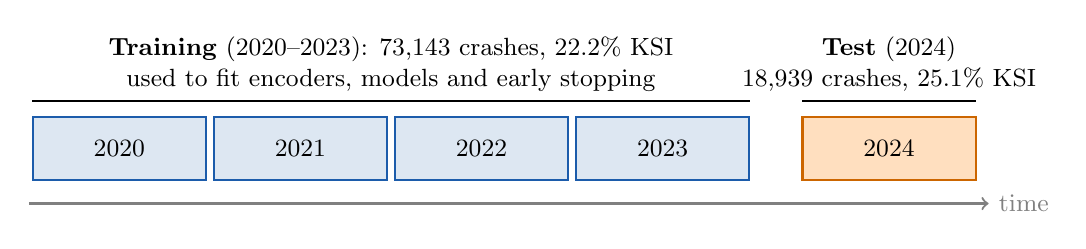
\begin{tikzpicture}[yr/.style={draw=accent, thick, minimum width=2.2cm, minimum height=0.8cm, font=\small},
                    x=2.3cm]
  \foreach \y/\lab in {0/2020,1/2021,2/2022,3/2023}{
    \node[yr, fill=accent!15] at (\y,0) {\lab};
  }
  \node[yr, fill=orange!25, draw=orange!80!black] at (4.25,0) {2024};
  \draw[decorate, thick] (-0.48,0.6) -- (3.48,0.6) node[midway, above, font=\small, align=center]
       {\textbf{Training} (2020--2023): 73,143 crashes, 22.2\% KSI\\used to fit encoders, models and early stopping};
  \draw[thick] (3.77,0.6) -- (4.73,0.6) node[midway, above, font=\small, align=center] {\textbf{Test} (2024)\\18,939 crashes, 25.1\% KSI};
  \draw[->, thick, gray] (-0.5,-0.7) -- (4.8,-0.7) node[right, font=\small] {time};
\end{tikzpicture}
\caption{Temporal validation design. All fitting (encoders, coefficients, trees, early stopping) uses 2020--2023 only; 2024 is scored once.}
\label{fig:split}
\end{figure}

\textbf{Controls against optimistic results.}
\begin{itemize}
  \item \emph{No information from the test year} is used for fitting. Encoders and models sit in one pipeline fitted
        on the training rows, and gradient boosting's early-stopping set is carved out of the training years.
  \item \emph{Hyperparameters were fixed in advance} (Table~\ref{tab:hyper}) and not tuned against 2024, so the test score
        is an honest estimate. Tuning will use the training years only (see below).
  \item \emph{Leaky and target-defining fields are excluded} (Table~\ref{tab:excluded}). A comparison run that includes
        \emph{Street lighting} is reported separately to show the size of the leakage effect.
\end{itemize}

\textbf{Evaluation metrics.} Because only about a quarter of crashes are KSI, accuracy would be misleading: the
baseline that never predicts KSI is 75\% accurate in 2024 but useless. The metrics below are used instead
\parencite{he2009,saito2015,fawcett2006}. Let TP, FP, TN and FN be the true/false positives and negatives when a
crash is labelled high-risk if $\hat{p}_i \geq 0.5$.
\begin{itemize}
  \item \textbf{ROC-AUC} (discrimination): the probability that a randomly chosen KSI crash receives a higher
        predicted risk than a randomly chosen non-KSI crash. 0.5 is random, 1.0 is perfect. It does not depend on
        the threshold.
  \item \textbf{PR-AUC} (average precision): the area under the precision--recall curve. Its random baseline equals
        the KSI prevalence (0.251 in 2024), so it is more sensitive than ROC-AUC to performance on the minority
        class \parencite{saito2015}.
  \item \textbf{Recall (sensitivity)} $= \text{TP}/(\text{TP}+\text{FN})$: the share of actual KSI crashes the model
        flags. For road safety, missing a severe crash is the costlier error, so recall is prioritised.
  \item \textbf{Precision} $= \text{TP}/(\text{TP}+\text{FP})$: the share of flagged crashes that really were KSI,
        which indicates how many resources would go to false alarms.
  \item \textbf{Fatal crashes flagged}: recall measured on fatal crashes only, the outcome stakeholders care
        most about.
  \item \textbf{Calibration by risk decile}: crashes are sorted into ten equal groups by $\hat{p}$, and the mean
        predicted risk is compared with the observed KSI rate in each group. A well-ranked model shows observed rates
        rising steadily across deciles. A well-calibrated one has predicted and observed rates that match
        \parencite{niculescu2005}.
\end{itemize}
The 0.5 threshold is applied to the class-weighted model's output, which places it roughly at the training
prevalence. In practice the threshold can be moved to trade recall against precision, for example to fit an
agency's inspection budget.

\textbf{Criteria for a \enquote{good} model.} A model is judged suitable for this case study if it meets the criteria
in Table~\ref{tab:criteria}. Together they cover performance, generalisation, stability and interpretability.
Common rules of thumb treat a ROC-AUC of 0.7--0.8 as acceptable and 0.8--0.9 as excellent discrimination
\parencite{hosmer2013}.

\begin{table}[H]
\centering
\caption{Criteria used to identify a good model, with the evidence for the two candidate models (2024 test year unless stated).}
\label{tab:criteria}
\footnotesize
\begin{tabularx}{\textwidth}{@{}P{3.0cm}P{3.6cm}LL@{}}
\toprule
\textbf{Criterion} & \textbf{Test} & \textbf{Logistic regression} & \textbf{Gradient boosting} \\
\midrule
Better than chance & ROC-AUC $> 0.5$; PR-AUC $>$ prevalence (0.251) & 0.742; 0.483 \checkmark & 0.749; 0.498 \checkmark \\
Acceptable discrimination & ROC-AUC $\geq 0.7$ \parencite{hosmer2013} & \checkmark & \checkmark \\
Catches severe crashes & High recall, especially on fatal crashes & 65\% KSI; 85\% fatal & 67\% KSI; 85\% fatal \\
No overfitting & Small gap between train and test ROC-AUC & 0.742 vs 0.742 & 0.764 vs 0.749 \\
Stable over time & Leave-one-year-out ROC-AUC within 2020--2023 & 0.730--0.748 & 0.734--0.754 \\
Ranks risk usefully & Observed KSI rises across risk deciles & -- & 5.5\% $\rightarrow$ 60.7\% \\
Calibrated probabilities & Predicted $\approx$ observed per decile & Not yet (class weighting) & Not yet (top decile 0.79 vs 0.61) \\
Interpretable & Effects explainable to stakeholders & Odds ratios & Permutation importance only \\
\bottomrule
\end{tabularx}
\end{table}

\textbf{Stability check.} To check that the 2024 result is not a one-off, each model was also re-fitted four times
on the training years, each time holding out one year (2020, 2021, 2022 or 2023) and scoring it
(Listing~\ref{lst:model}, lines 100--108). ROC-AUC stayed between 0.730 and 0.754 across held-out years for
both models. The lowest score was for 2021, the COVID-affected year, and the 2024 test score lies inside this
range, so performance is consistent over time. The next stage will use this same leave-one-year-out scheme on
the training years to tune hyperparameters and the decision threshold, keeping 2024 untouched.

\textbf{How feature influence is measured.} For logistic regression, influence is read from the odds ratios
(Equation~\ref{eq:logit}). For gradient boosting, which has no coefficients, \textbf{permutation importance} is used
\parencite{breiman2001}: each predictor's values are randomly shuffled in the 2024 data, five times, and the
average drop in ROC-AUC is recorded. A large drop means the model relies on that predictor (Listing~\ref{lst:model},
line 146).

\subsection{Suitability for the case study}
\begin{itemize}
  \item \textbf{Logistic regression} is the most suitable \emph{primary} model for this case study. The
        stakeholders are public agencies that must justify their investment decisions, and odds ratios
        translate directly into program priorities. It performs only 0.007 AUC below gradient boosting
        (Section~\ref{sec:prelim}).
  \item \textbf{Gradient boosting} works best as a \emph{check} on the logistic model. Its small gain suggests
        that severity is driven mostly by additive main effects in this feature set. Its importance ranking
        independently confirms the logistic model's drivers.
  \item \textbf{Limitations of both:} predicted probabilities are inflated by class weighting and need
        recalibration before they are reported as risks \parencite{niculescu2005}. Neither model accounts for
        the unobserved heterogeneity that the accident-research literature stresses. Ordered and random-parameters
        models are the natural extension for the full five-level severity scale
        \parencite{savolainen2011,mannering2014}.
  \item \textbf{Spatial models} (density-based clustering of KSI crashes) are better suited than classifiers to
        Q3 and are planned for the next stage.
\end{itemize}

% =================================================================
\section{Data visualisation and communication of results}
\label{sec:viz}

Each visual was chosen to answer one question for one audience, and all were produced with Matplotlib
\parencite{hunter2007} using a single consistent design system. Table~\ref{tab:viz} maps each visual to its
question and audience.

\begin{table}[H]
\centering
\caption{Visualisations, the questions they answer and their intended audience.}
\label{tab:viz}
\small
\begin{tabularx}{\textwidth}{@{}P{4.3cm}P{1.3cm}LP{3.1cm}@{}}
\toprule
\textbf{Visual (technique)} & \textbf{Q} & \textbf{Purpose} & \textbf{Audience} \\
\midrule
Severity bar chart (Fig.~\ref{fig:severity}) & -- & Class balance; justifies the KSI target & Analysts \\
Yearly trend lines (Fig.~\ref{fig:trend}) & Q4 & COVID dip and post-2022 rise & TfNSW, public \\
Day $\times$ time heatmaps (Fig.~\ref{fig:heatmap}) & Q4 & Volume against severity by time & Police \\
Speed limit $\times$ region lines (Fig.~\ref{fig:speed}) & Q2 & Regional gap at equal speed & TfNSW, councils \\
Impact-type 100\% stacked bars (Fig.~\ref{fig:impact}) & Q1 & Severity share by crash mechanism & All \\
Hexbin maps (Fig.~\ref{fig:map}) & Q3 & Where crashes and severe crashes are & Councils, TfNSW \\
ROC/PR curves (Fig.~\ref{fig:roc}) & Q1 & Model performance & Analysts \\
Odds ratios and importance (Figs.~\ref{fig:odds}, \ref{fig:perm}) & Q1 & Drivers of severity & Policy makers \\
\bottomrule
\end{tabularx}
\end{table}

Key design choices:
\begin{itemize}
  \item \textbf{Rates alongside counts.} Volume and severity often point in different directions. The heatmaps
        (Fig.~\ref{fig:heatmap}) and maps (Fig.~\ref{fig:map}) pair a count view with a KSI-share view, so that
        \enquote{where crashes are common} is not mistaken for \enquote{where crashes are dangerous}.
  \item \textbf{Hexagonal binning for 92,000 points.} Plotting each crash as a point would create heavy overplotting
        along the coast. Hexbins aggregate points into equal-area cells \parencite{carr1987}. A logarithmic
        colour scale keeps sparse regional cells visible next to Sydney cells with thousands of crashes. Cells
        with fewer than 15 crashes are hidden on the KSI-share map to avoid unstable rates.
  \item \textbf{Geographic context.} ABS state, Greater Sydney and LGA boundaries \parencite{abs_asgs}, plus labelled
        markers for Sydney, Newcastle and Wollongong, let non-technical readers orient themselves.
  \item \textbf{Accessible colour.} Single-hue sequential scales encode magnitude. Categorical series use a
        palette checked for colour-vision-deficiency separation, and series are also labelled directly or with a
        legend, so colour is never the only cue.
  \item \textbf{Small-sample suppression and annotation.} Groups with fewer than 100 crashes are hidden in the
        speed chart, and bar charts are annotated with sample sizes.
  \item \textbf{Models explained in policy terms.} Odds ratios are shown on a log scale centred at 1, so effects
        that raise and lower risk appear symmetrically.
\end{itemize}

% =================================================================
\section{Preliminary results}
\label{sec:prelim}

\subsection{Data characterisation and distributions}

\textbf{Severity.} Of the 92,082 crashes from 2020 to 2024, 32.0\% were non-casualty tow-aways, 28.4\% moderate
injury, 16.8\% minor injury, 21.3\% serious injury and 1.5\% fatal (1,388 crashes, 1,507 deaths;
Figure~\ref{fig:severity}). The KSI target therefore has a prevalence of 22.8\%. Most crashes involve two
traffic units (59\%), and 29\% are single-vehicle crashes.

\begin{figure}[H]
\centering
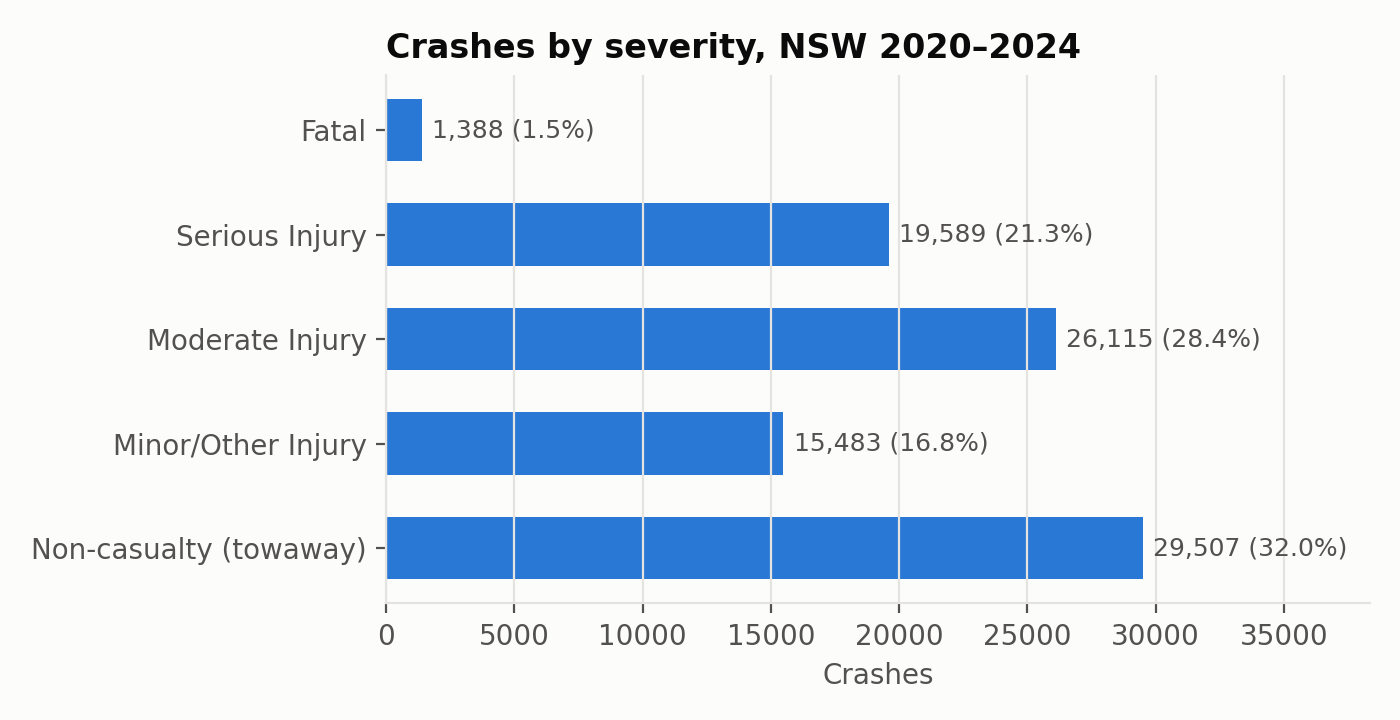
\includegraphics[width=0.72\textwidth]{01_severity_distribution.png}
\caption{Distribution of crashes by severity, NSW 2020--2024.}
\label{fig:severity}
\end{figure}

\textbf{Trend.} Fatal crashes held at around 260 a year in 2020--2022 and rose to around 300 in 2023--2024.
Serious-injury crashes fell in 2021, during COVID-19 lockdowns, and then rose 37\% to 4,459 in 2024, while
moderate, minor and tow-away crashes stayed flat (Figure~\ref{fig:trend}). Severe crashes are therefore
increasing, not crashes overall, which moves NSW away from its 2030 targets.

\begin{figure}[H]
\centering
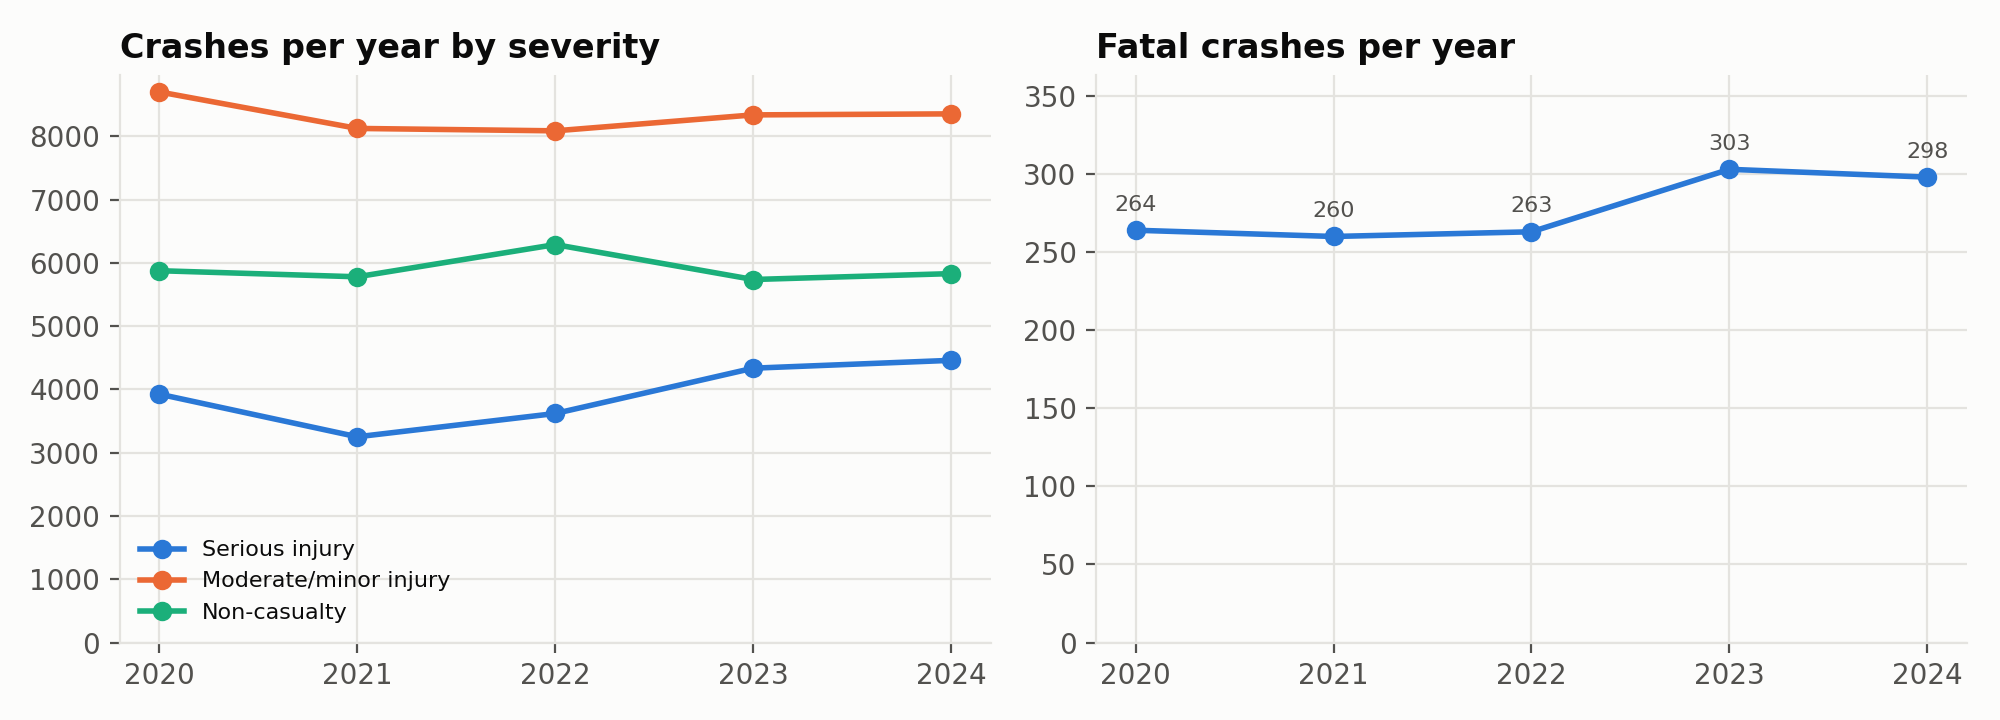
\includegraphics[width=\textwidth]{02_yearly_trend.png}
\caption{Crashes per year by severity (left) and fatal crashes per year (right).}
\label{fig:trend}
\end{figure}

\textbf{Time of day and week.} Crash volume peaks on weekday afternoons; Friday 16:00--17:59 is the busiest
slot, with 2,304 crashes. Severity follows a different pattern: the highest KSI shares occur on
\emph{weekend mornings}, reaching 31\% on Sunday 10:00--11:59 and 29\% on Sunday 08:00--09:59, against about
20\% in the weekday peak (Figure~\ref{fig:heatmap}). Congested peak traffic produces many low-speed crashes,
while lighter weekend traffic, often on recreational and regional routes, produces fewer but more severe ones.

\begin{figure}[H]
\centering
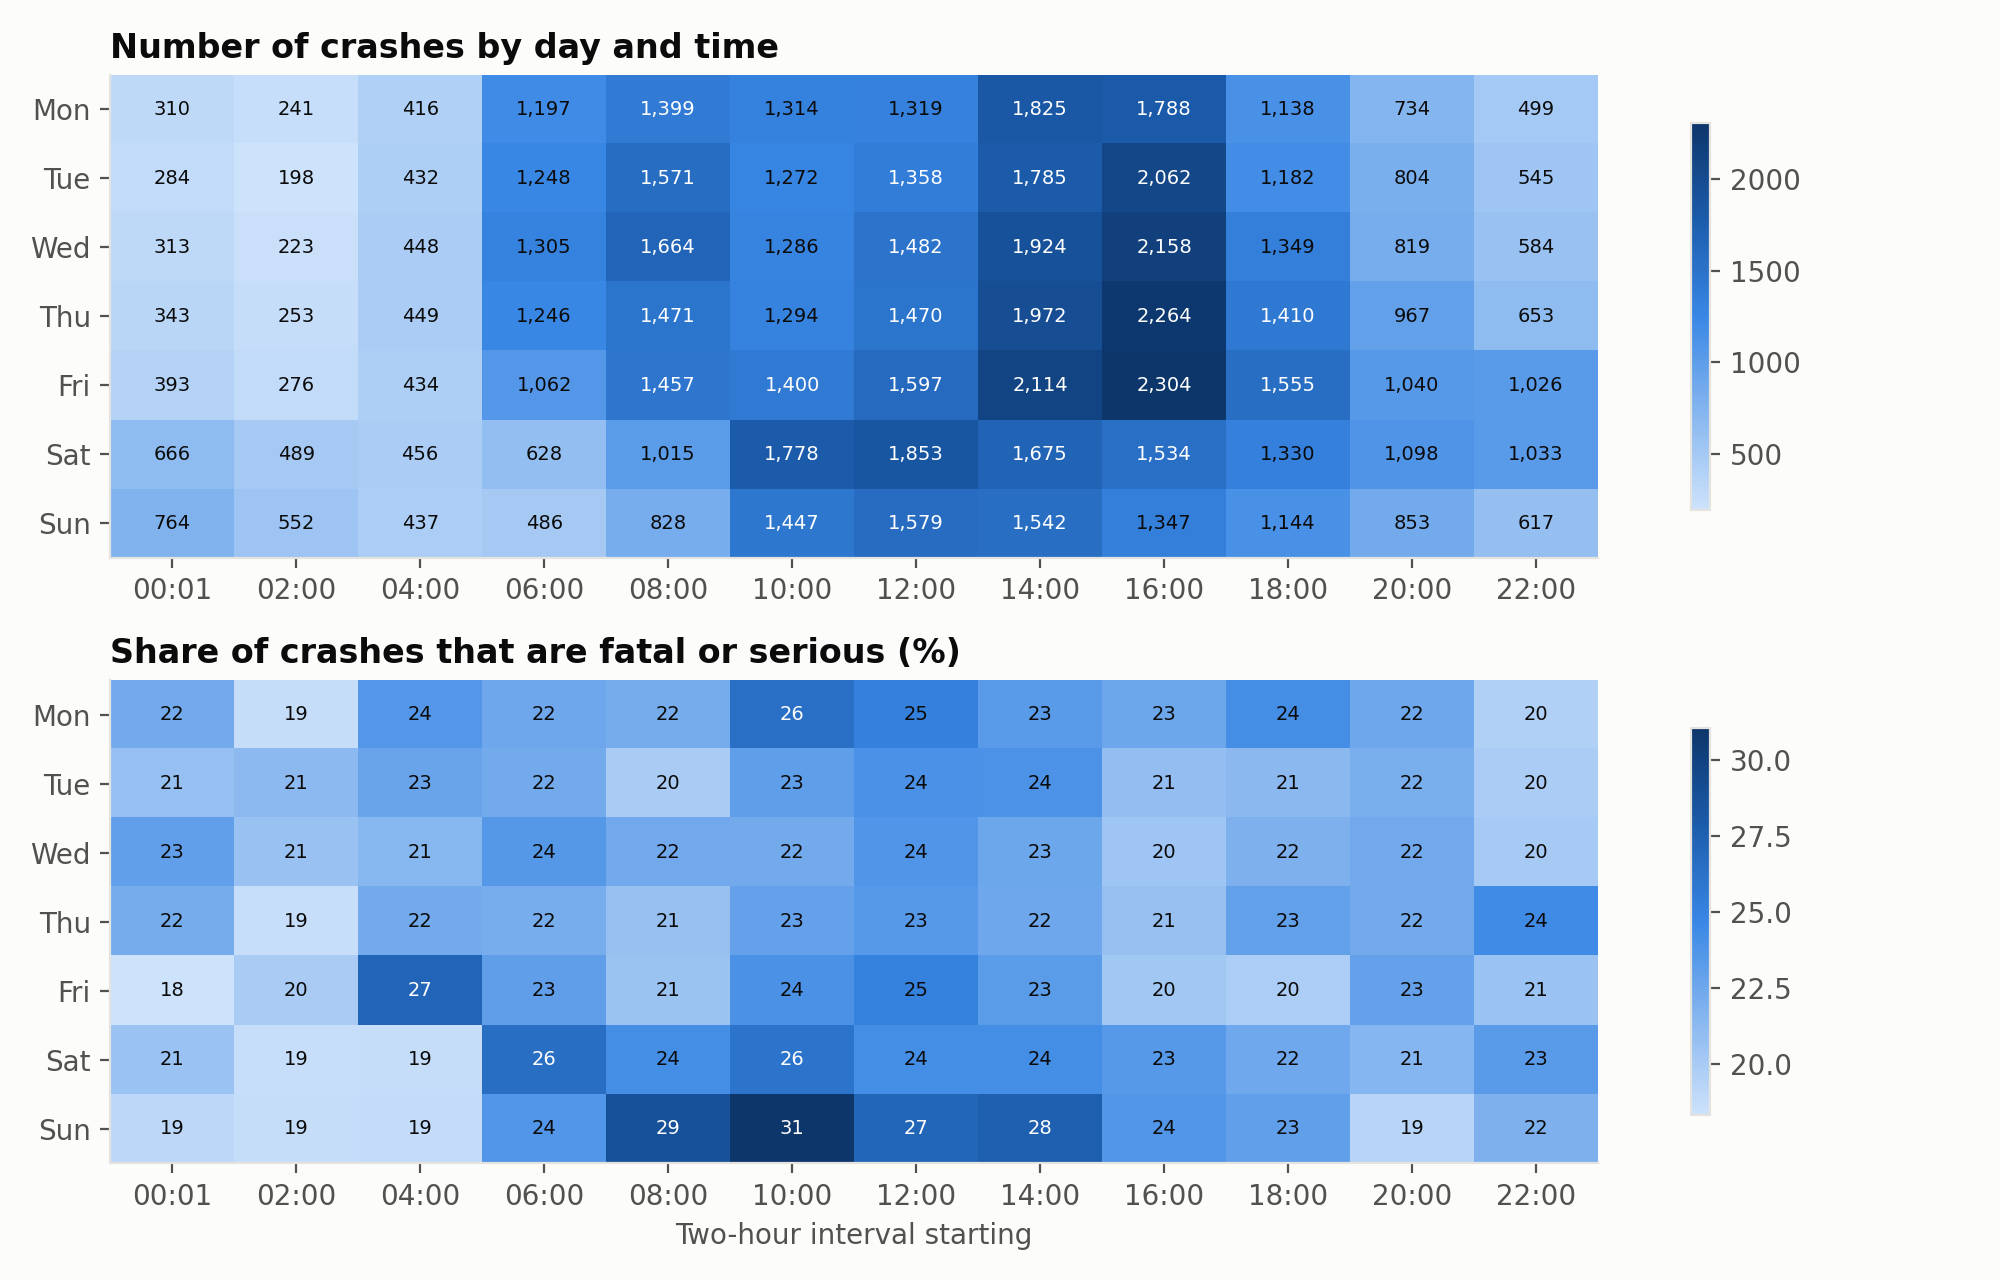
\includegraphics[width=0.95\textwidth]{03_time_heatmaps.png}
\caption{Crash counts (top) and share of crashes that are fatal or serious (bottom) by day and two-hour interval.}
\label{fig:heatmap}
\end{figure}

\textbf{Regional gap (Q2).} Table~\ref{tab:region} shows that regional rural NSW has 12.7\% of crashes but 39.2\%
of deaths, with a fatal-crash rate five times that of the metropolitan conurbation. This matches TfNSW's statement
that more than two-thirds of deaths occur on country roads \parencite{tfnsw_actionplan}. Even at the same speed
limit, crashes outside the conurbation are more severe (Figure~\ref{fig:speed}): at 100\,km/h, 5.0\% are fatal
against 1.4\% in the metro areas, and at 80\,km/h, 3.4\% against 1.6\%. Crash mechanism contributes to the gap:
74.8\% of rural crashes are single-vehicle crashes (metro: 18.2\%), and 45.1\% are vehicle--object impacts
(metro: 14.1\%).

\begin{table}[H]
\centering
\caption{Crashes, deaths and severity by region, 2020--2024.}
\label{tab:region}
\small
\begin{tabularx}{\textwidth}{@{}P{5.6cm}RRRRR@{}}
\toprule
\textbf{Region} & \textbf{Crashes} & \textbf{Share of crashes} & \textbf{Deaths} & \textbf{Share of deaths} & \textbf{Fatal rate} \\
\midrule
Greater Sydney / Newcastle / Wollongong & 62,551 & 67.9\% & 580 & 38.5\% & 0.9\% \\
Regional urban & 17,821 & 19.4\% & 337 & 22.4\% & 1.7\% \\
Regional rural & 11,690 & 12.7\% & 590 & 39.2\% & 4.5\% \\
\bottomrule
\end{tabularx}
\end{table}

\begin{figure}[H]
\centering
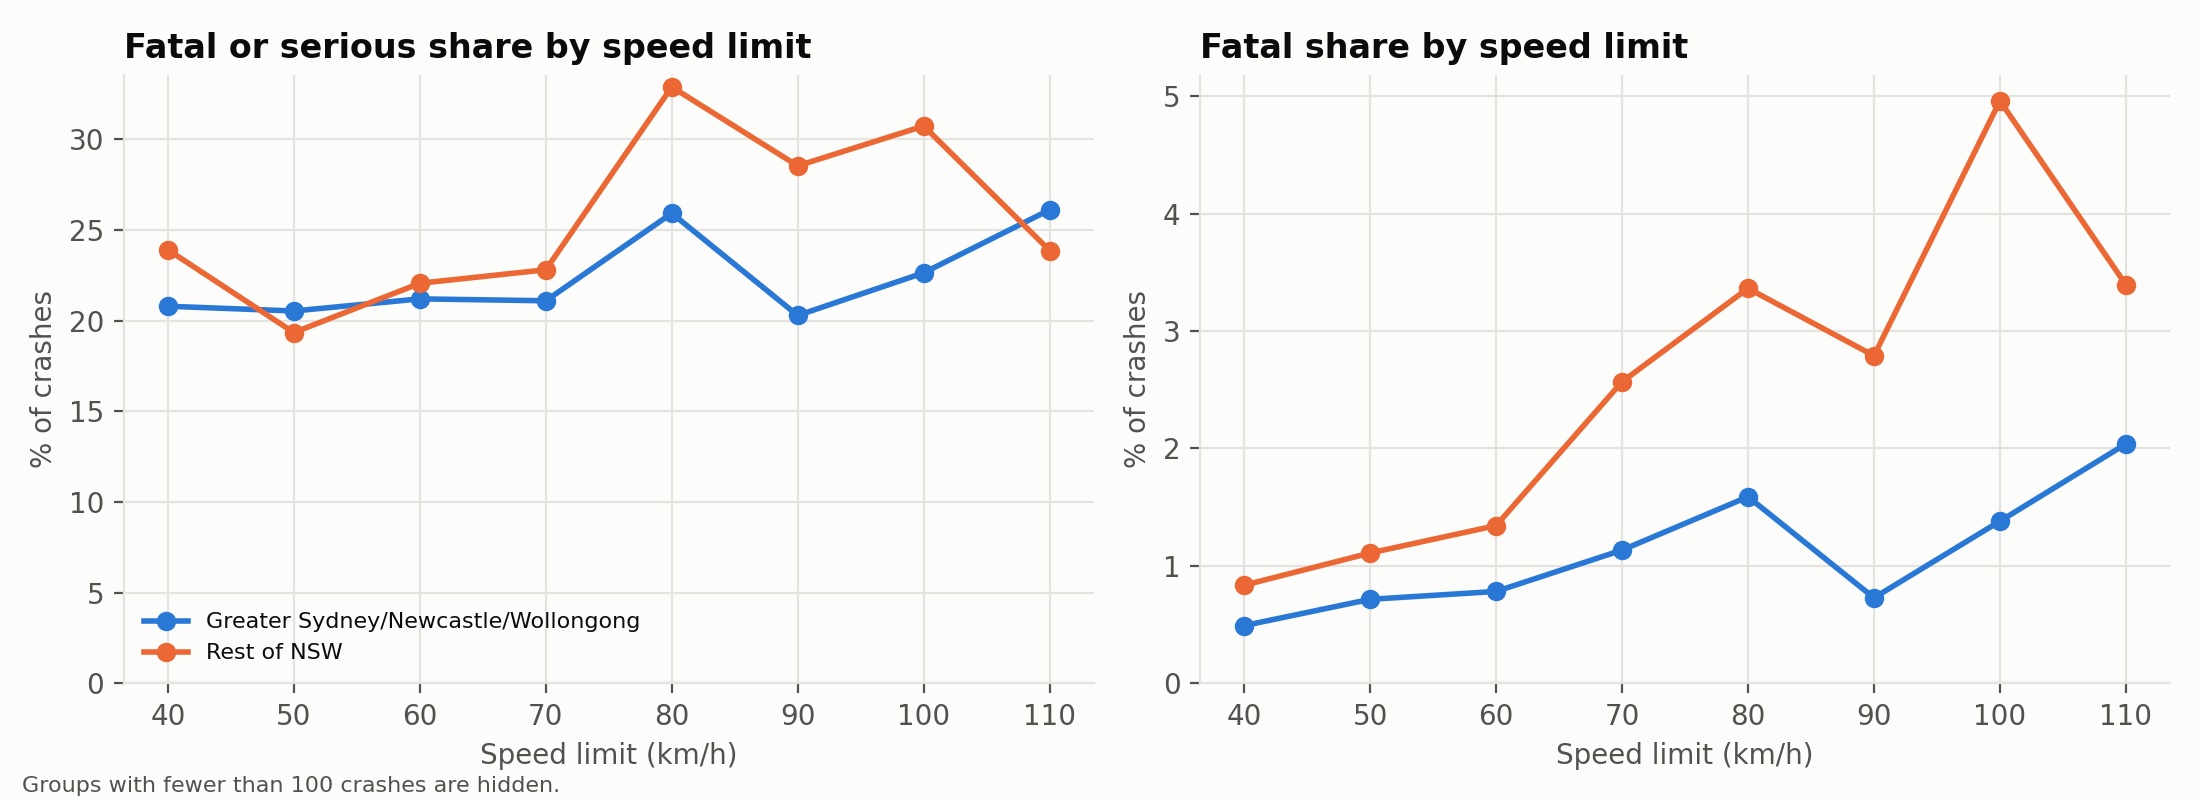
\includegraphics[width=\textwidth]{04_severity_by_speed_region.png}
\caption{KSI share (left) and fatal share (right) by speed limit, metropolitan conurbation against the rest of NSW.}
\label{fig:speed}
\end{figure}

\textbf{Crash mechanism.} Pedestrian (47\% KSI), person--object (46\%), head-on (39\%) and rollover (32\%) crashes
are the most severe, and rear-end crashes the least (13\%; Figure~\ref{fig:impact}). Head-on crashes have the highest
fatal share, at 6.4\%.

\begin{figure}[H]
\centering
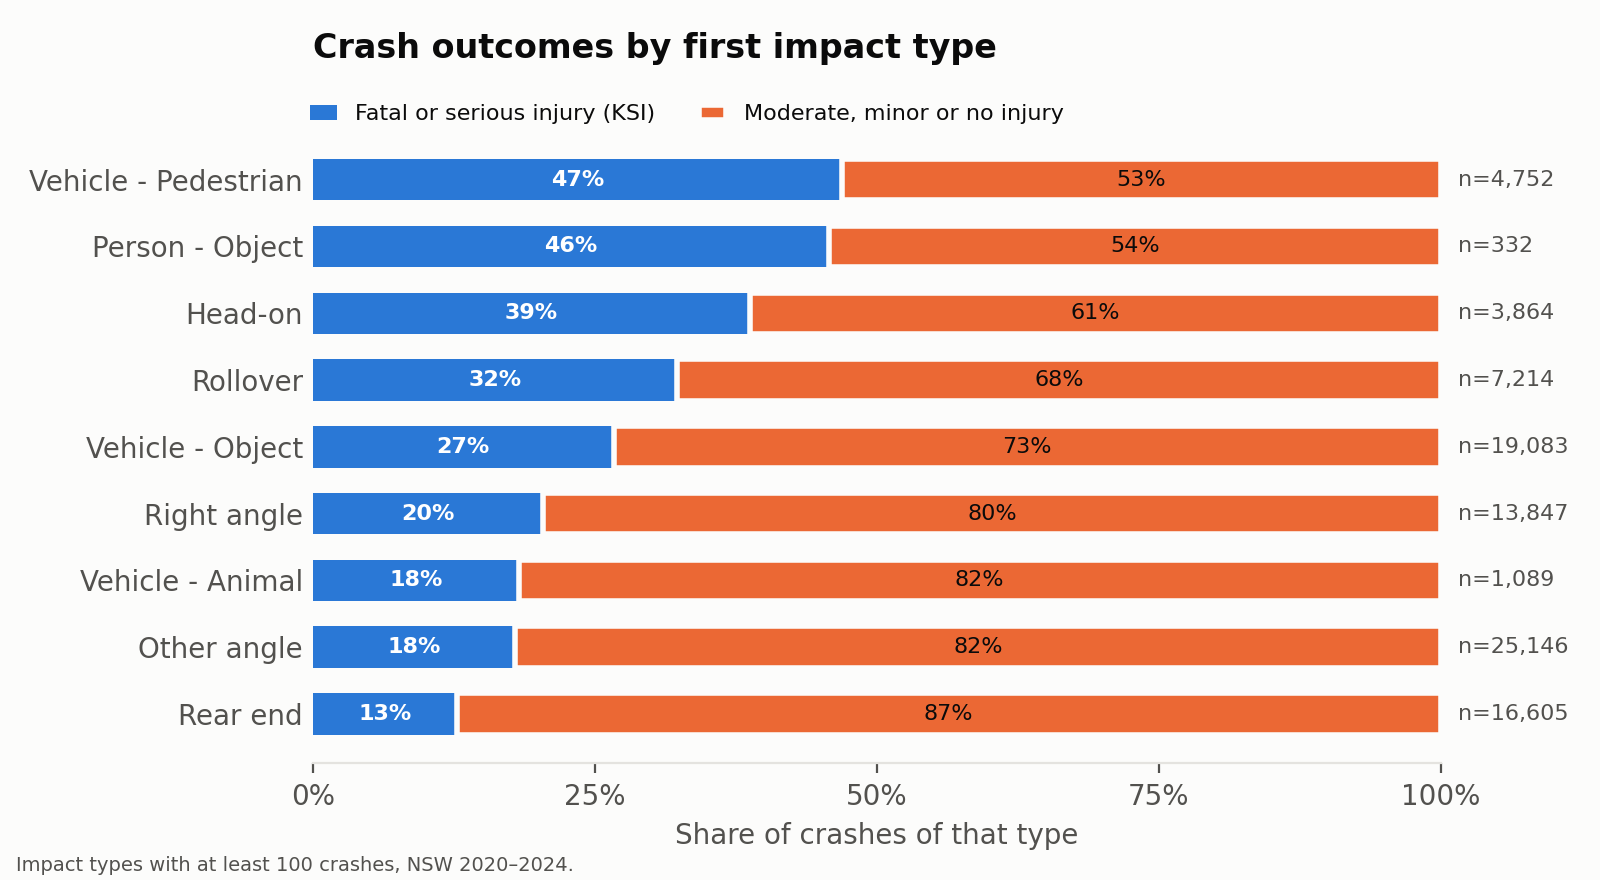
\includegraphics[width=0.72\textwidth]{05_ksi_by_impact_type.png}
\caption{Crash outcomes by first impact type: share of crashes that were fatal or serious (blue) against moderate, minor or no injury (orange). Impact types with at least 100 crashes.}
\label{fig:impact}
\end{figure}

\textbf{Spatial distribution (Q3).} Crashes follow the population and the highway network, with the densest
cells in Sydney and along the Pacific, Hume and New England corridors (Figure~\ref{fig:map}, left). Within Greater
Sydney, KSI shares appear higher on the urban fringe and along major arterials than in the dense inner
suburbs (Figure~\ref{fig:map}, right). By count, the LGAs with the most KSI crashes are Central Coast (1,068),
Canterbury-Bankstown (990) and Blacktown (823).

\begin{figure}[H]
\centering
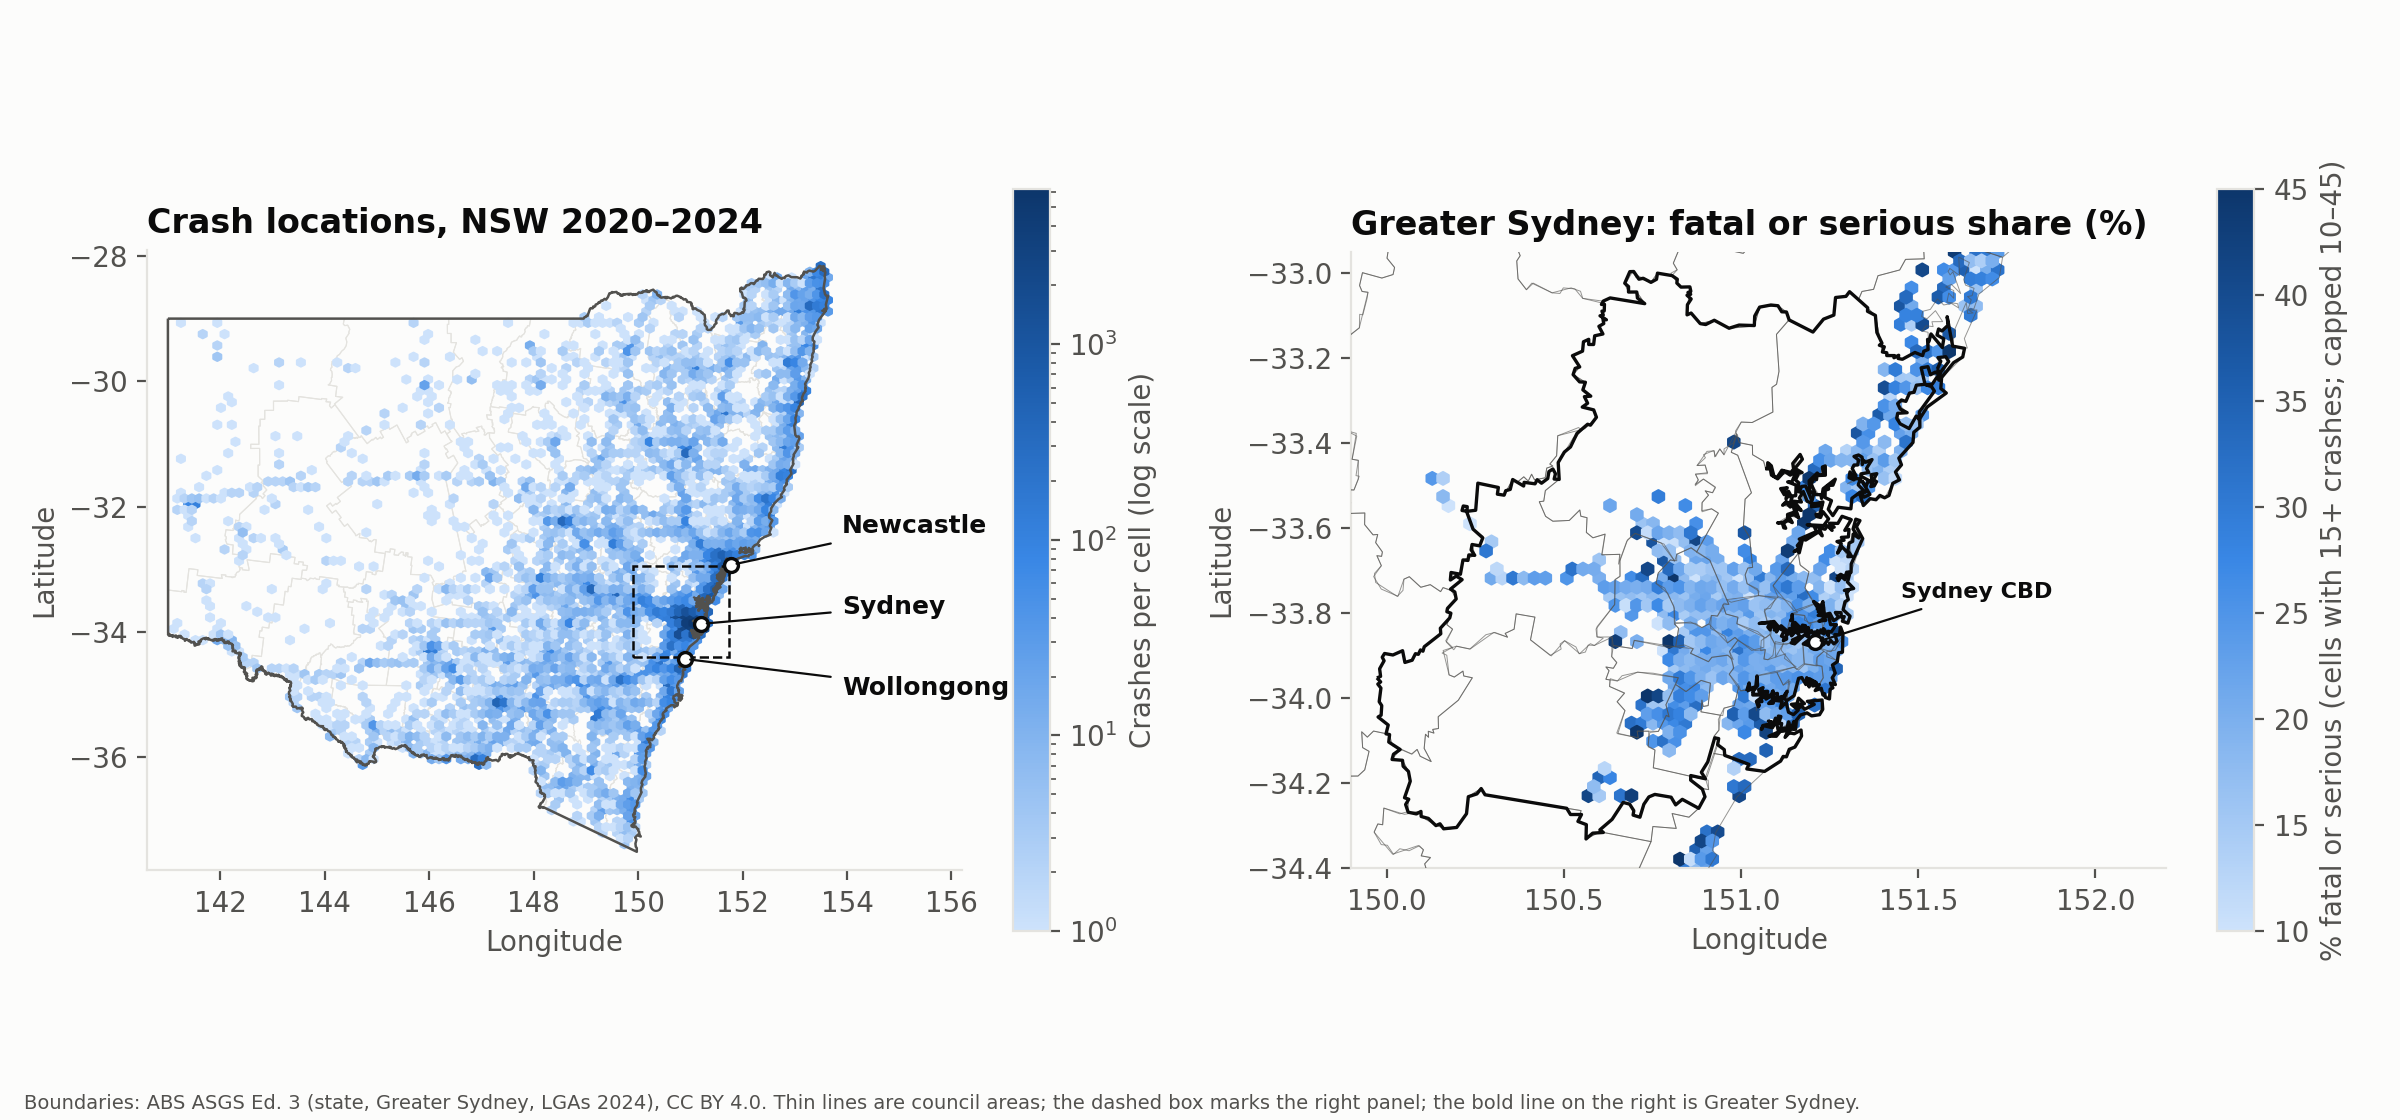
\includegraphics[width=\textwidth]{06_crash_map.png}
\caption{Crash density across NSW, log scale (left), and KSI share within Greater Sydney (right). Boundaries: ABS ASGS Edition 3.}
\label{fig:map}
\end{figure}

\subsection{Initial modelling results}

Table~\ref{tab:results} reports test-set performance on 2024 crashes. Both models clearly outperform the baseline.
Gradient boosting achieves a ROC-AUC of 0.749 and a PR-AUC of 0.498, double the 0.251 that random ranking would
give. Logistic regression is within 0.007 AUC. At the default threshold, the models identify about two-thirds of
KSI crashes and 85\% of fatal crashes. The ROC and PR curves almost coincide (Figure~\ref{fig:roc}).

\begin{table}[H]
\centering
\caption{Model performance on the 2024 test set (18,939 crashes, 25.1\% KSI).}
\label{tab:results}
\small
\begin{tabularx}{\textwidth}{@{}P{5.4cm}RRRRR@{}}
\toprule
\textbf{Model} & \textbf{ROC-AUC} & \textbf{PR-AUC} & \textbf{KSI recall} & \textbf{KSI precision} & \textbf{Fatal crashes flagged} \\
\midrule
Majority-class baseline & 0.500 & 0.251 & 0.00 & -- & 0\% \\
Logistic regression & 0.742 & 0.483 & 0.65 & 0.44 & 85\% \\
Gradient boosting & \textbf{0.749} & \textbf{0.498} & 0.67 & 0.43 & 85\% \\
\midrule
\emph{Gradient boosting incl.\ Street lighting (leaky)} & \emph{0.809} & \emph{0.553} & \emph{0.81} & \emph{0.45} & \emph{95\%} \\
\bottomrule
\end{tabularx}
\end{table}

\begin{figure}[H]
\centering
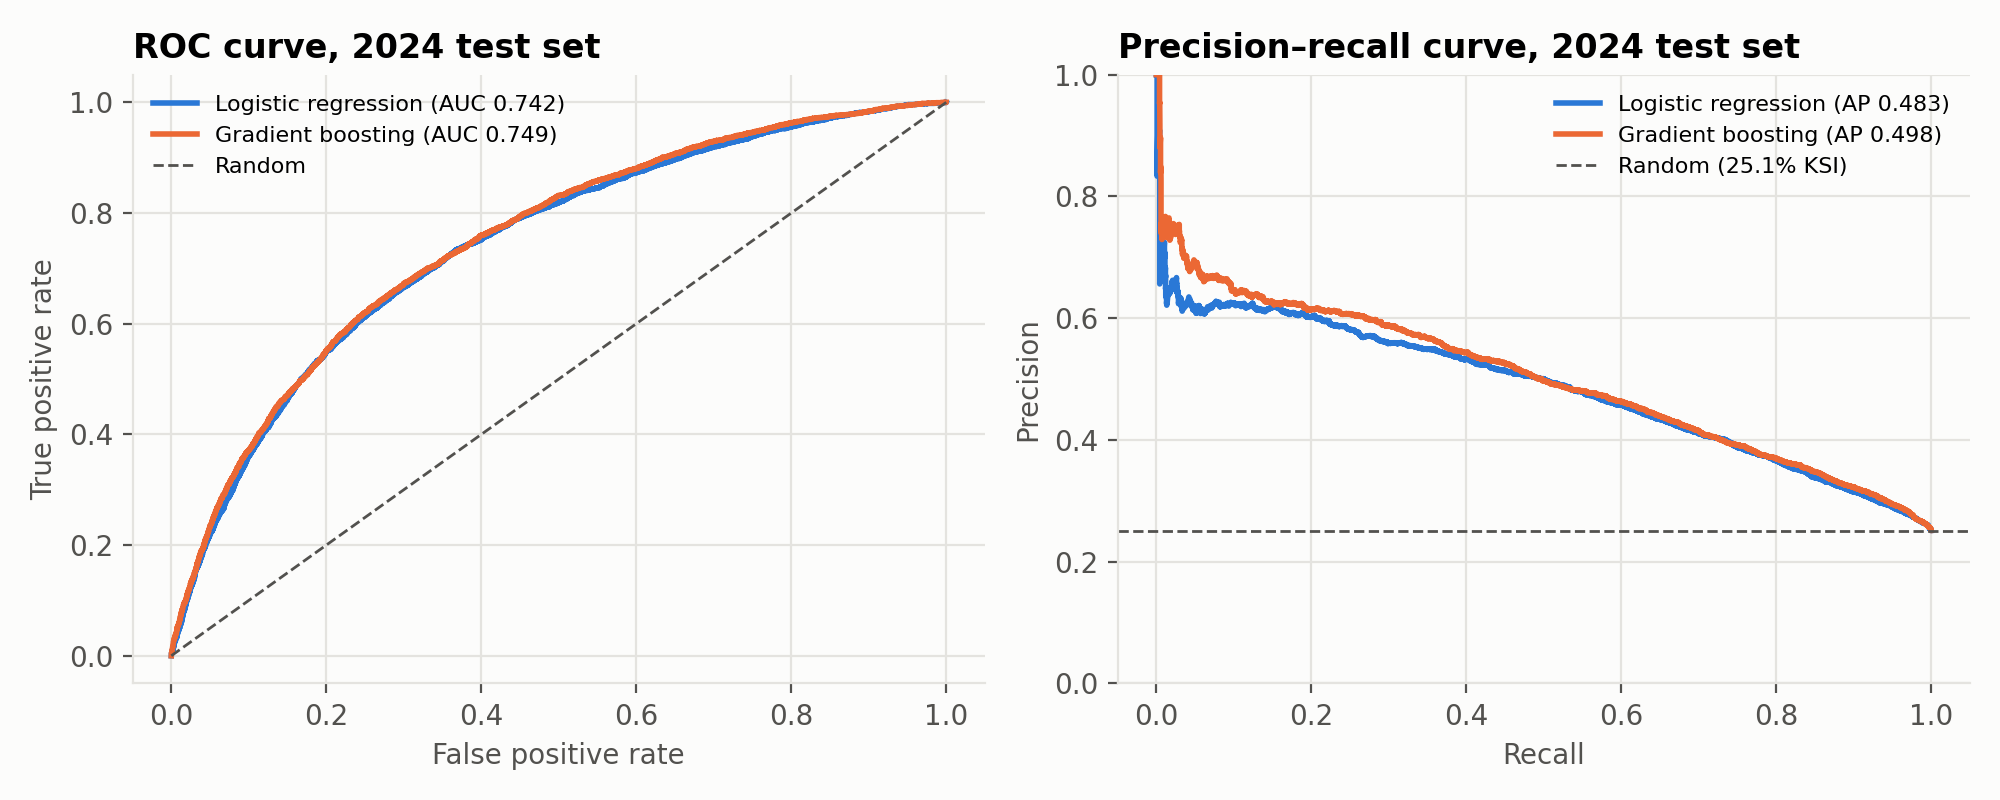
\includegraphics[width=\textwidth]{07_model_roc_pr.png}
\caption{ROC (left) and precision--recall (right) curves on the 2024 test set.}
\label{fig:roc}
\end{figure}

\textbf{Risk ranking.} When 2024 crashes are sorted into deciles by predicted risk, the actual KSI rate rises
steadily from 5.5\% in the lowest decile to 60.7\% in the highest, an eleven-fold spread. However, the top decile's
mean predicted probability is 0.79, which confirms the over-estimation expected from class weighting and the need
for recalibration.

\textbf{Leakage check.} Adding \emph{Street lighting} raises ROC-AUC to 0.809 and fatal-crash recall to 95\%
(Table~\ref{tab:results}, last row). In that run, \emph{Street lighting} becomes by far the most important feature,
which only makes sense as a recording artefact. This demonstrates how the data-quality issue in
Section~\ref{sec:data} would inflate apparent performance, and why the leaky feature was removed.

\textbf{Drivers of severity (Q1).} The two models agree on the main drivers (Figures~\ref{fig:odds} and~\ref{fig:perm}):
\begin{itemize}
  \item \textbf{Motorcycle involvement} is the strongest factor (odds ratio $\approx$5.7; largest permutation
        importance). 49\% of motorcycle crashes are KSI, compared with 19\% of other crashes.
  \item \textbf{Vulnerable road users}: pedestrian ($\approx$4.4), cyclist ($\approx$4.3) and person--object
        ($\approx$4.4) involvement, and motorised mobility scooters ($\approx$7.2, though based on few cases).
  \item \textbf{Roadside objects and crash mechanism}: hitting a tree or pole ($\approx$2.5), head-on impact
        ($\approx$2.0) and heavy-vehicle involvement ($\approx$1.8).
  \item \textbf{Speed environment}: 100--110\,km/h zones ($\approx$1.5--1.7). Rear-end crashes ($\approx$0.46), animal
        strikes ($\approx$0.42) and 40\,km/h zones ($\approx$0.53) are associated with lower severity.
  \item Weather, day of week and school-zone status contribute almost nothing once these factors are known.
\end{itemize}
Remaining \enquote{unknown} categories (for example \emph{Natural lighting: Unknown}, odds ratio $\approx$0.17) show
the same recording effect and will be handled in the next stage. These are associations and should not be read as
causal effects.

\begin{figure}[H]
\centering
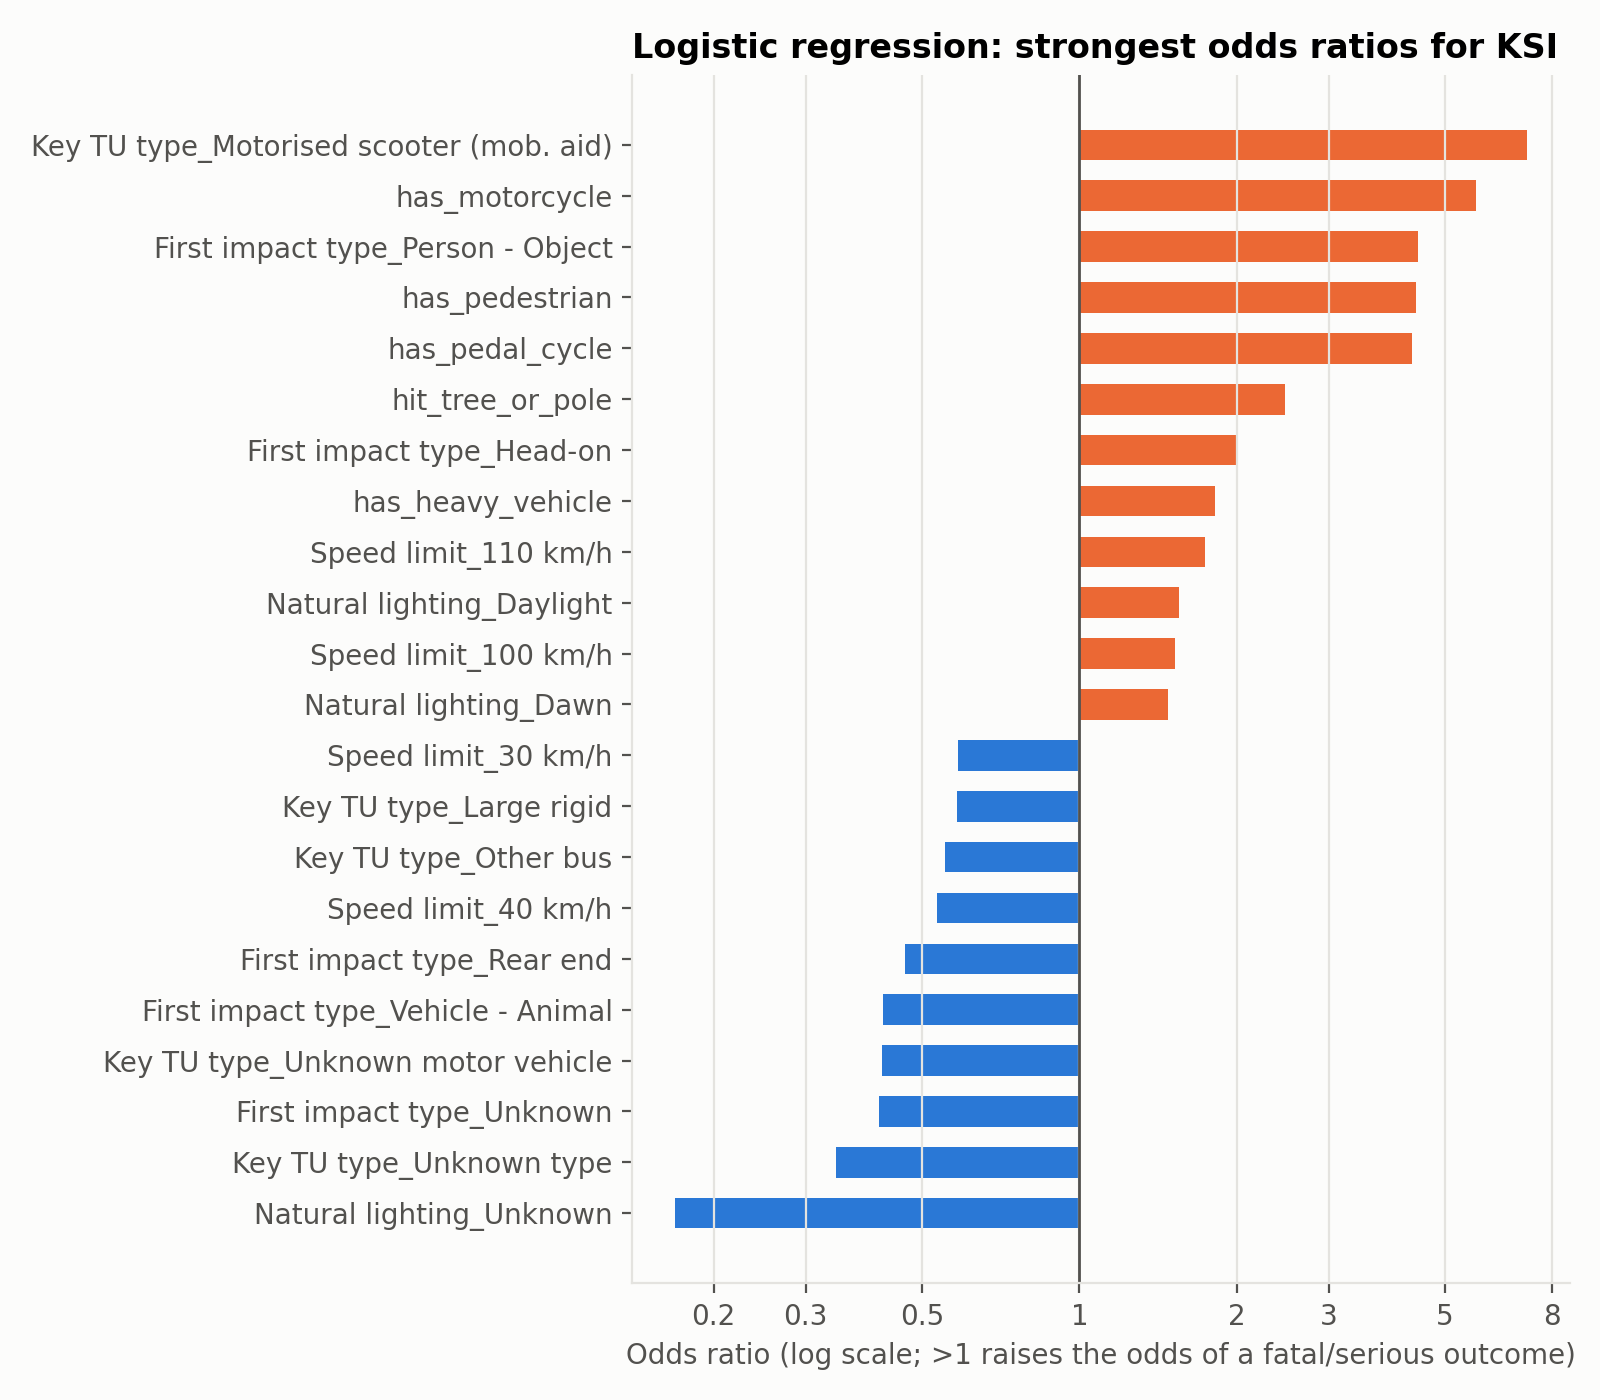
\includegraphics[width=0.78\textwidth]{08_logreg_odds_ratios.png}
\caption{Strongest logistic-regression odds ratios for a KSI outcome (log scale).}
\label{fig:odds}
\end{figure}

\begin{figure}[H]
\centering
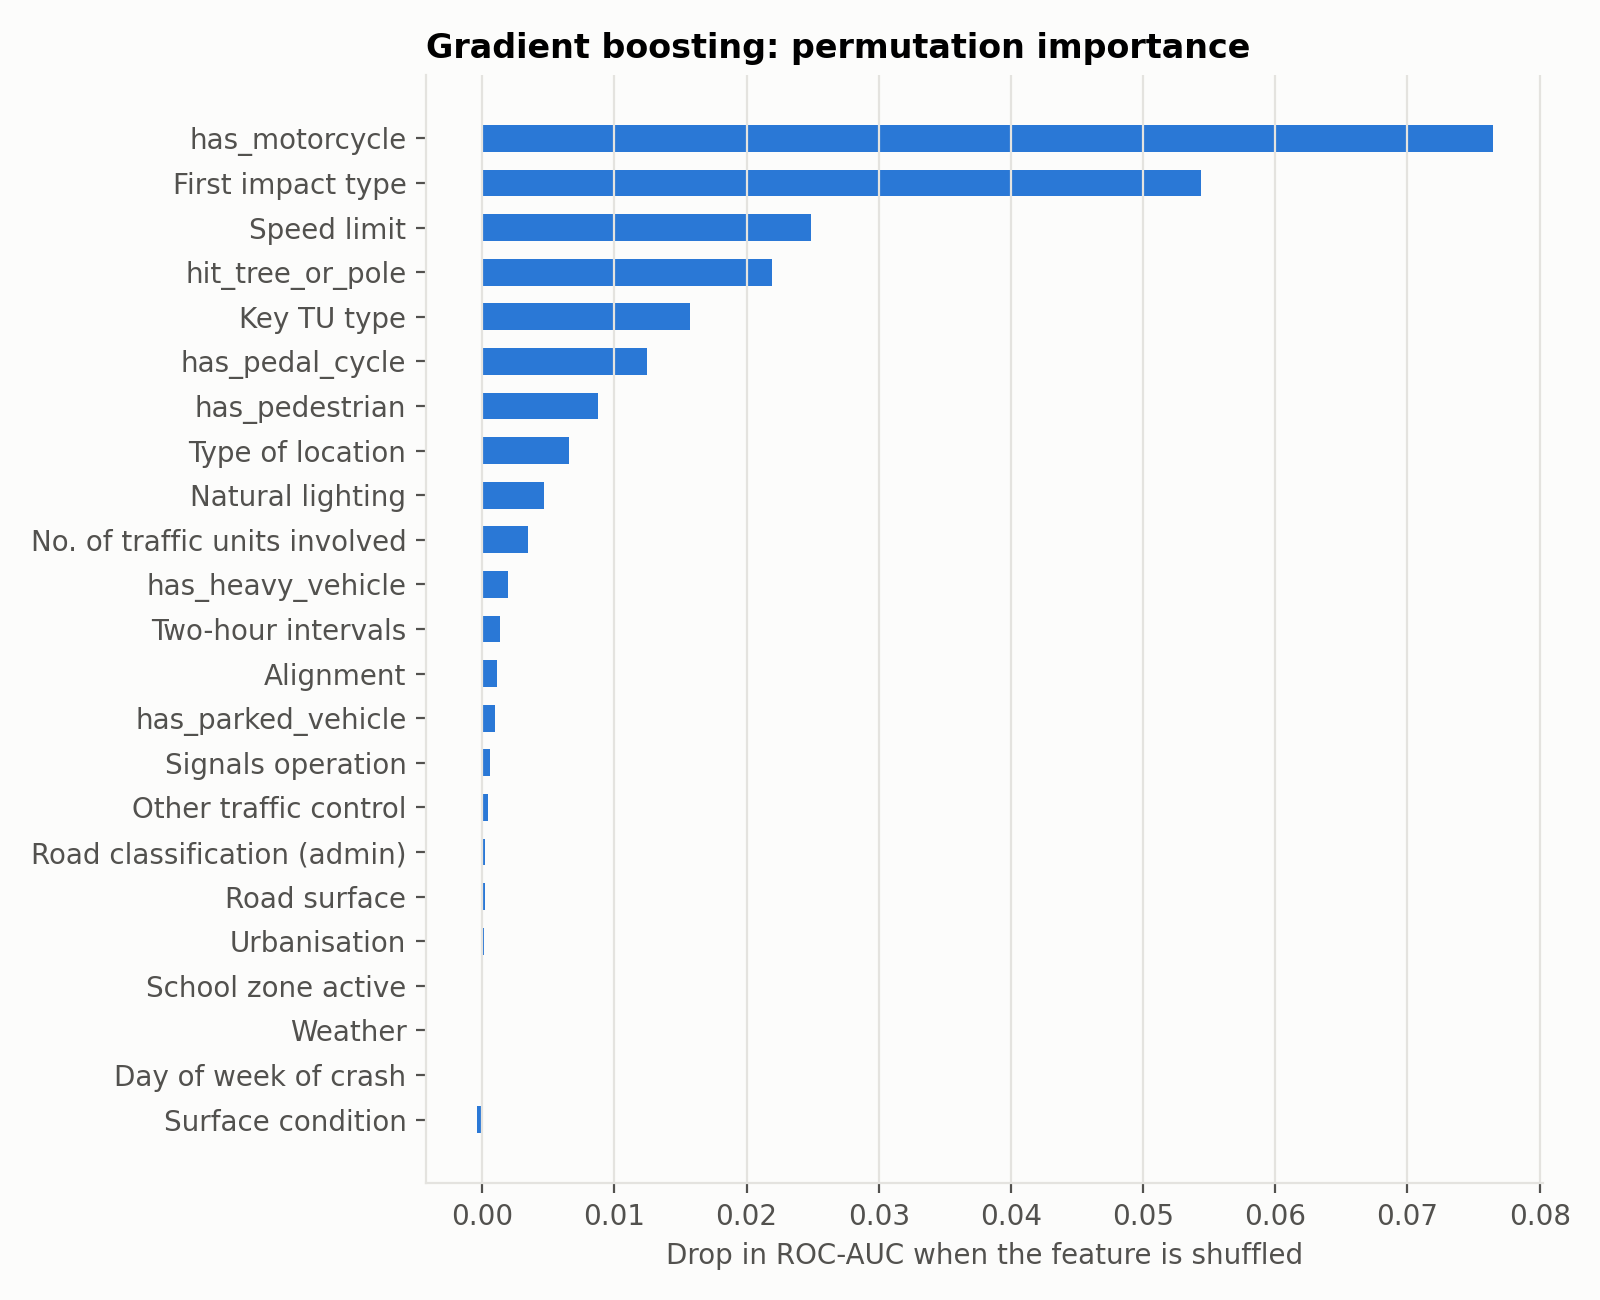
\includegraphics[width=0.78\textwidth]{09_gb_permutation_importance.png}
\caption{Gradient-boosting permutation importance (drop in test ROC-AUC when a feature is shuffled).}
\label{fig:perm}
\end{figure}

\subsection{Interpretation and next steps}
A ROC-AUC of about 0.75 is moderate, and the ceiling reflects the data rather than the model: the main
determinants of injury severity, such as travel speed, restraint use, impairment, occupant age and vehicle
safety rating, are not in the open release. Even so, the models separate low- and high-risk crash profiles
clearly and give consistent, policy-relevant drivers. The next stage will:
\begin{enumerate}
  \item recode structural blanks, treat the remaining \enquote{unknown} levels, and recalibrate probabilities;
  \item add ABS population data to compare LGAs by per-capita KSI rate (Q3);
  \item model the regional gap directly, controlling for speed, mechanism and vehicle mix (Q2);
  \item apply density-based clustering to KSI crash locations to identify hotspots (Q3);
  \item extend to the full ordered severity scale and a fatal-only model, and check stability with rolling-year validation.
\end{enumerate}

% =================================================================
\newpage
\printbibliography[heading=bibintoc,title={References}]

% =================================================================
\newpage
\appendix
\section{How the models work}
\label{app:models}

This appendix explains, step by step, how the two predictive models in Section~\ref{sec:model} turn the predictors
of a crash into a risk of a killed-or-seriously-injured (KSI) outcome. It lists every predictor each model uses and
works through two real crashes from the 2024 test year. The code that builds and runs the models is in
Appendix~\ref{app:code}.

\subsection{What goes in and what comes out}
Both models receive the same 23 predictors for every crash (Table~\ref{tab:predictors}): 16 categorical
descriptions of the road, environment, time and crash mechanism, plus 7 crash-level counts and flags derived
from the TRAFFIC UNIT table. Both return one number per crash: an estimated probability $\hat{p}$ that the crash is
KSI. A crash is labelled \emph{high risk} if $\hat{p} \geq 0.5$.

The two models read the predictors differently:
\begin{itemize}
  \item \textbf{Logistic regression} cannot read text categories. Each categorical predictor is therefore
        \emph{one-hot encoded}: \emph{Speed limit}, for example, becomes 12 columns (\texttt{Speed limit\_50 km/h},
        \texttt{Speed limit\_60 km/h}, \ldots), and a crash has a 1 in the column for its speed limit and 0 in the others.
        Levels seen fewer than 50 times in training are pooled into one \enquote{infrequent} column per predictor.
        The 16 categorical predictors become 121 columns, and with the 7 numeric and binary predictors the model sees
        \textbf{128 input columns} (Table~\ref{tab:allcoef}).
  \item \textbf{Gradient boosting} uses the 23 predictors directly. Categories are stored as integer codes, and the
        trees split them as groups of categories (for example \{Head-on, Rollover\} against the rest).
\end{itemize}

\subsection{Logistic regression, step by step}
\label{app:lr}

\textbf{Step 1 --- add up a score.} Every input column $j$ has a learned weight $\beta_j$. For a given crash, the model
starts from an intercept $\beta_0$ and adds the weight of every column that is switched on (multiplied by its value
for the numeric predictor). The total is the crash's \emph{log-odds score} $z$:
\[
  z = \beta_0 + \beta_{\text{speed}=100} + \beta_{\text{impact}=\text{Vehicle--Object}} + \cdots + \beta_{\text{units}} \times (\text{no.\ of units}) + \beta_{\text{motorcycle}} \times 1 .
\]
A positive weight pushes the crash towards KSI, and a negative weight pushes it away.

\textbf{Step 2 --- turn the score into a probability.} The logistic (sigmoid) function squeezes any score into the range
0 to 1: $\hat{p} = 1/(1+e^{-z})$. A score of 0 gives 0.5, large positive scores approach 1, and large negative scores
approach 0.

\textbf{Step 3 --- learn the weights.} The weights are chosen to make the training crashes' observed outcomes as likely
as possible (maximum likelihood), which means minimising the log-loss in Equation~\ref{eq:lrloss}. Two adjustments are
made. First, each KSI crash counts about 2.25 times and each non-KSI crash about 0.64 times (class weighting), so the
minority class is not ignored. Second, an L2 penalty ($C=0.5$) pulls weights towards zero, which stops rare categories
from receiving extreme weights. The optimiser (L-BFGS) adjusts all 129 numbers (128 weights plus the intercept)
together until the loss stops improving; this took 92 iterations.

\textbf{Step 4 --- read the weights.} Raising $e$ to a weight gives an \emph{odds ratio}. An odds ratio of 5.72 for
\texttt{has\_motorcycle} means that, other predictors being equal, the odds of KSI are 5.72 times higher when a motorcycle
is involved. Because every level of a categorical predictor has its own column and the penalty shrinks them, the
weights should be compared \emph{between levels of the same predictor}. For example, \emph{Rear end} ($-0.77$) against
\emph{Head-on} ($+0.69$) shows how much the impact type changes the score. A level should not be read in isolation.
Table~\ref{tab:allcoef} lists every weight and odds ratio the model learned.

\textbf{Worked example.} Table~\ref{tab:example_inputs} shows two real 2024 crashes: a motorcycle that left a curved
100\,km/h country road and struck an object (crash~1360953, actual outcome: serious injury), and a two-car
rear-end crash on a 60\,km/h divided road in metropolitan Sydney (crash~1343582, actual outcome: moderate injury).
Each was chosen as the most typical member (median predicted risk) of its crash profile in 2024.
Table~\ref{tab:example_lr} shows how logistic regression adds up their scores.

\begin{table}[H]
\centering
\caption{Predictor values of the two worked-example crashes (2024 test year).}
\label{tab:example_inputs}
\footnotesize
\begin{tabularx}{\textwidth}{@{}P{4.6cm}LL@{}}
\toprule
\textbf{Predictor} & \textbf{High-risk example (\#1360953)} & \textbf{Low-risk example (\#1343582)} \\
\midrule
Urbanisation & Country non-urban & Sydney metro. area \\
Speed limit & 100 km/h & 60 km/h \\
Weather & Unknown & Fine \\
Natural lighting & Daylight & Daylight \\
Surface condition & Dry & Dry \\
Road surface & Sealed & Sealed \\
Alignment & Curved & Curved \\
Type of location & 2-way undivided & Divided road \\
Road classification (admin) & Regional & State \\
First impact type & Vehicle - Object & Rear end \\
Key TU type & Motorcycle & Car (sedan/hatch) \\
Two-hour intervals & 10:00 - 11:59 & 12:00 - 13:59 \\
Day of week of crash & Wednesday & Sunday \\
School zone active & Not a school zone & Not a school zone \\
Signals operation & Nil & Nil \\
Other traffic control & No traffic controls & No traffic controls \\
No. of traffic units involved & 1 & 2 \\
has\_pedestrian & 0 & 0 \\
has\_motorcycle & 1 & 0 \\
has\_pedal\_cycle & 0 & 0 \\
has\_heavy\_vehicle & 0 & 0 \\
hit\_tree\_or\_pole & 0 & 0 \\
has\_parked\_vehicle & 0 & 0 \\
\midrule
Actual outcome & Serious Injury (KSI = 1) & Moderate Injury (KSI = 0) \\
\bottomrule
\end{tabularx}
\end{table}

\begin{table}[H]
\centering
\caption{Logistic regression score for the two example crashes: each predictor's contribution
$\beta_j x_j$ to the log-odds $z$, then the probability.}
\label{tab:example_lr}
\footnotesize
\begin{tabular}{@{}lrr@{}}
\toprule
\textbf{Contribution to $z$ from\ldots} & \textbf{High-risk} & \textbf{Low-risk} \\
\midrule
Intercept $\beta_0$ & -0.448 & -0.448 \\
Urbanisation & -0.072 & -0.016 \\
Speed limit & +0.421 & -0.069 \\
Weather & -0.049 & +0.032 \\
Natural lighting & +0.440 & +0.440 \\
Surface condition & -0.031 & -0.031 \\
Road surface & -0.203 & -0.203 \\
Alignment & -0.141 & -0.141 \\
Type of location & +0.111 & -0.112 \\
Road classification (admin) & -0.107 & -0.193 \\
First impact type & +0.045 & -0.768 \\
Key TU type & +0.193 & +0.083 \\
Two-hour intervals & -0.023 & -0.006 \\
Day of week of crash & -0.081 & -0.047 \\
School zone active & -0.212 & -0.212 \\
Signals operation & +0.128 & +0.128 \\
Other traffic control & -0.073 & -0.073 \\
No. of traffic units involved & +0.248 & +0.497 \\
has\_pedestrian & +0.000 & +0.000 \\
has\_motorcycle & +1.743 & +0.000 \\
has\_pedal\_cycle & +0.000 & +0.000 \\
has\_heavy\_vehicle & +0.000 & +0.000 \\
hit\_tree\_or\_pole & +0.000 & +0.000 \\
has\_parked\_vehicle & +0.000 & +0.000 \\
\midrule
\textbf{Log-odds score $z$} & \textbf{+1.890} & \textbf{-1.139} \\
\textbf{Probability $\hat{p} = 1/(1+e^{-z})$} & \textbf{0.869} & \textbf{0.242} \\
Label at threshold 0.5 & High risk & Not high risk \\
\bottomrule
\end{tabular}
\end{table}

For the motorcycle crash, the single largest push comes from \texttt{has\_motorcycle} ($+1.74$), helped by the
100\,km/h limit ($+0.42$). The score of $+1.89$ gives a probability of 0.87, and the crash is correctly flagged as
high risk. For the rear-end crash, the impact type pulls the score down strongly ($-0.77$), giving $z = -1.14$ and
$\hat{p} = 0.24$, so it is correctly not flagged. Both probabilities are higher than the true risk because of class
weighting (Section~\ref{sec:validation}); the \emph{ranking} of the two crashes is what matters.

\subsection{Gradient boosting, step by step}
\label{app:gb}

Gradient boosting builds its prediction from many small decision trees, each correcting the mistakes of the ones
before it \parencite{friedman2001,ke2017}.

\textbf{Step 1 --- start from a neutral guess.} Every crash starts with the same score $F_0$. With balanced class
weights this corresponds to a probability of about 0.5.

\textbf{Step 2 --- measure the errors.} For each training crash, the model computes how far its current probability is
from the truth (the gradient of the log-loss: roughly $y_i - \hat{p}_i$). KSI crashes with low predicted risk have
large positive errors, and non-KSI crashes with high predicted risk have large negative ones.

\textbf{Step 3 --- fit a small tree to the errors.} A decision tree with at most 31 leaves is grown to separate crashes
with similar errors. At each split, the tree tries every predictor. For numeric predictors it tries thresholds over at most
255 histogram bins; for categorical ones, groupings of categories. It keeps the split that best reduces the error.
A tree might, for instance, first split on \texttt{has\_motorcycle}, then on \emph{First impact type} $\in$
\{Head-on, Vehicle--Object, Rollover\}, then on \emph{Speed limit} $\geq$ 90\,km/h. Each leaf stores a correction value.

\textbf{Step 4 --- take a small step.} Each crash's score is moved by its leaf's correction multiplied by the learning
rate $\eta = 0.05$. Small steps mean no single tree dominates, which makes the model more robust.

\textbf{Step 5 --- repeat, and stop at the right time.} Steps 2--4 are repeated, with each new tree focusing on what is
still wrong. scikit-learn sets aside 10\% of the training crashes and stops once 10 consecutive trees fail to improve
the loss on them (early stopping). Training stopped after \textbf{105 trees}.

\textbf{Step 6 --- predict.} A new crash is passed down all 105 trees; its leaf corrections are added to $F_0$, and the
total score is turned into a probability with the same sigmoid function as logistic regression
(Equation~\ref{eq:gbm}).

Because a path down a tree combines several predictors (motorcycle \emph{and} 100\,km/h \emph{and} curved road), gradient
boosting learns interactions automatically. The cost is that there is no single weight per predictor to read.
Instead, \textbf{permutation importance} measures how much the 2024 ROC-AUC drops when one predictor's values are randomly
shuffled (Table~\ref{tab:allperm}).

\textbf{Worked example.} Table~\ref{tab:example_gb} follows the same two crashes as the trees are added. Both start near
0.5. The motorcycle crash's risk climbs as successive trees recognise its high-risk profile, while the rear-end crash's
risk falls. Most of the movement happens in the first 50 trees, which is why early stopping ended training at 105.

\begin{table}[H]
\centering
\caption{Gradient boosting probability for the two example crashes after $m$ trees.}
\label{tab:example_gb}
\footnotesize
\begin{tabular}{@{}rrr@{}}
\toprule
\textbf{Trees used ($m$)} & \textbf{High-risk example} & \textbf{Low-risk example} \\
\midrule
1 & 0.517 & 0.485 \\
5 & 0.575 & 0.430 \\
10 & 0.631 & 0.377 \\
25 & 0.737 & 0.289 \\
50 & 0.796 & 0.241 \\
105 & 0.802 & 0.224 \\
\midrule
Label at threshold 0.5 & High risk & Not high risk \\
\bottomrule
\end{tabular}
\end{table}

\begin{table}[H]
\centering
\caption{Gradient boosting permutation importance for all 23 predictors (mean drop in 2024 ROC-AUC over five shuffles).
Values near zero mean the model barely relies on the predictor; a small negative value is random noise.}
\label{tab:allperm}
\footnotesize
\begin{tabular}{@{}rlr@{}}
\toprule
\textbf{Rank} & \textbf{Predictor} & \textbf{Drop in ROC-AUC} \\
\midrule
1 & has\_motorcycle & 0.0764 \\
2 & First impact type & 0.0544 \\
3 & Speed limit & 0.0248 \\
4 & hit\_tree\_or\_pole & 0.0220 \\
5 & Key TU type & 0.0158 \\
6 & has\_pedal\_cycle & 0.0125 \\
7 & has\_pedestrian & 0.0088 \\
8 & Type of location & 0.0066 \\
9 & Natural lighting & 0.0047 \\
10 & No. of traffic units involved & 0.0035 \\
11 & has\_heavy\_vehicle & 0.0019 \\
12 & Two-hour intervals & 0.0014 \\
13 & Alignment & 0.0012 \\
14 & has\_parked\_vehicle & 0.0010 \\
15 & Signals operation & 0.0006 \\
16 & Other traffic control & 0.0004 \\
17 & Road classification (admin) & 0.0002 \\
18 & Road surface & 0.0002 \\
19 & Urbanisation & 0.0001 \\
20 & School zone active & 0.0001 \\
21 & Weather & 0.0000 \\
22 & Day of week of crash & 0.0000 \\
23 & Surface condition & -0.0004 \\
\bottomrule
\end{tabular}
\end{table}

\subsection{Comparing the two models}
\begin{table}[H]
\centering
\caption{How the two models differ in practice.}
\label{tab:modelcompare}
\footnotesize
\begin{tabularx}{\textwidth}{@{}P{3.2cm}LL@{}}
\toprule
 & \textbf{Logistic regression} & \textbf{Gradient boosting} \\
\midrule
Form of the model & One weighted sum of 128 inputs & Sum of 105 small trees \\
Predictor interactions & Only if added by hand & Learned automatically \\
Explaining a prediction & Exact: add up the contributions (Table~\ref{tab:example_lr}) & Indirect: importance, staged predictions \\
2024 test ROC-AUC & 0.742 & 0.749 \\
Best use here & Primary model for stakeholders & Check on whether non-linear effects are missed \\
\bottomrule
\end{tabularx}
\end{table}

\subsection{Complete list of logistic regression inputs}
Table~\ref{tab:allcoef} lists all 128 encoded inputs, grouped by the original predictor, with the learned weight $\beta_j$
and odds ratio $e^{\beta_j}$. Within each predictor, levels are sorted from the most to the least severe association.

{\scriptsize
\setlength{\tabcolsep}{4pt}
\begin{longtable}{@{}p{3.6cm}p{6.6cm}rr@{}}
\caption{All logistic regression inputs with learned weights and odds ratios.}\label{tab:allcoef}\\
\toprule
\textbf{Predictor} & \textbf{Level / encoded column} & \textbf{$\beta_j$} & \textbf{Odds ratio} \\
\midrule
\endfirsthead
\multicolumn{4}{@{}l}{\emph{Table~\ref{tab:allcoef} continued}}\\
\toprule
\textbf{Predictor} & \textbf{Level / encoded column} & \textbf{$\beta_j$} & \textbf{Odds ratio} \\
\midrule
\endhead
\bottomrule
\endfoot
Urbanisation & Wollongong met. area & -0.007 & 0.99 \\
 & Sydney metro. area & -0.016 & 0.98 \\
 & Newcastle met. area & -0.018 & 0.98 \\
 & Country urban & -0.032 & 0.97 \\
 & Country non-urban & -0.072 & 0.93 \\
 & (infrequent levels, $<$50 rows) & -0.248 & 0.78 \\
\addlinespace[2pt]
Speed limit & 110 km/h & +0.555 & 1.74 \\
 & 100 km/h & +0.421 & 1.52 \\
 & 80 km/h & +0.345 & 1.41 \\
 & 90 km/h & +0.217 & 1.24 \\
 & 70 km/h & +0.112 & 1.12 \\
 & 60 km/h & -0.069 & 0.93 \\
 & 10 km/h & -0.185 & 0.83 \\
 & (infrequent levels, $<$50 rows) & -0.257 & 0.77 \\
 & 50 km/h & -0.373 & 0.69 \\
 & 30 km/h & -0.532 & 0.59 \\
 & 40 km/h & -0.627 & 0.53 \\
\addlinespace[2pt]
Weather & Raining & +0.038 & 1.04 \\
 & Fine & +0.032 & 1.03 \\
 & Fog or mist & -0.001 & 1.00 \\
 & Overcast & -0.015 & 0.98 \\
 & Unknown & -0.049 & 0.95 \\
 & Other & -0.150 & 0.86 \\
 & Snowing & -0.247 & 0.78 \\
\addlinespace[2pt]
Natural lighting & Daylight & +0.440 & 1.55 \\
 & Dawn & +0.389 & 1.47 \\
 & Darkness & +0.328 & 1.39 \\
 & Dusk & +0.231 & 1.26 \\
 & Unknown & -1.781 & 0.17 \\
\addlinespace[2pt]
Surface condition & Unknown & +0.300 & 1.35 \\
 & Dry & -0.031 & 0.97 \\
 & Wet & -0.176 & 0.84 \\
 & Snow or ice & -0.487 & 0.61 \\
\addlinespace[2pt]
Road surface & Unknown & +0.031 & 1.03 \\
 & Sealed & -0.203 & 0.82 \\
 & Unsealed & -0.221 & 0.80 \\
\addlinespace[2pt]
Alignment & Curved & -0.141 & 0.87 \\
 & Straight & -0.252 & 0.78 \\
\addlinespace[2pt]
Type of location & Single limited access & +0.150 & 1.16 \\
 & Other & +0.141 & 1.15 \\
 & 2-way undivided & +0.111 & 1.12 \\
 & Multiple intersection & +0.085 & 1.09 \\
 & T-junction & +0.073 & 1.08 \\
 & Y-junction & +0.018 & 1.02 \\
 & X-intersection & +0.010 & 1.01 \\
 & Dual freeway & +0.001 & 1.00 \\
 & (infrequent levels, $<$50 rows) & -0.091 & 0.91 \\
 & Divided road & -0.112 & 0.89 \\
 & L-junction & -0.201 & 0.82 \\
 & 1-way street & -0.250 & 0.78 \\
 & Roundabout & -0.329 & 0.72 \\
\addlinespace[2pt]
Road classification (admin) & Local & -0.093 & 0.91 \\
 & Regional & -0.107 & 0.90 \\
 & State & -0.193 & 0.82 \\
\addlinespace[2pt]
First impact type & Person - Object & +1.492 & 4.44 \\
 & Head-on & +0.690 & 1.99 \\
 & Vehicle - Pedestrian & +0.244 & 1.28 \\
 & (infrequent levels, $<$50 rows) & +0.176 & 1.19 \\
 & Vehicle - Object & +0.045 & 1.05 \\
 & Rollover & +0.007 & 1.01 \\
 & Right angle & -0.166 & 0.85 \\
 & Other angle & -0.368 & 0.69 \\
 & Rear end & -0.768 & 0.46 \\
 & Vehicle - Animal & -0.863 & 0.42 \\
 & Unknown & -0.880 & 0.41 \\
\addlinespace[2pt]
Key TU type & Motorised scooter (mob. aid) & +1.972 & 7.18 \\
 & Passenger van & +0.379 & 1.46 \\
 & (infrequent levels, $<$50 rows) & +0.361 & 1.43 \\
 & Motorised push scooters & +0.225 & 1.25 \\
 & Motorcycle & +0.193 & 1.21 \\
 & Pedal cycle & +0.190 & 1.21 \\
 & Light truck utility(from 2018) & +0.109 & 1.11 \\
 & Station wagon & +0.100 & 1.11 \\
 & Light truck & +0.086 & 1.09 \\
 & Car (sedan/hatch) & +0.083 & 1.09 \\
 & 4 wheel drive / SUV & +0.046 & 1.05 \\
 & Motor scooter & +0.024 & 1.02 \\
 & Utility & -0.026 & 0.97 \\
 & STA bus & -0.219 & 0.80 \\
 & Semi-trailer & -0.413 & 0.66 \\
 & B-double (road train prior 98) & -0.435 & 0.65 \\
 & Large rigid & -0.540 & 0.58 \\
 & Other bus & -0.589 & 0.55 \\
 & Unknown motor vehicle & -0.867 & 0.42 \\
 & Unknown type & -1.070 & 0.34 \\
\addlinespace[2pt]
Two-hour intervals & (infrequent levels, $<$50 rows) & +0.049 & 1.05 \\
 & 20:00 - 21:59 & +0.005 & 1.00 \\
 & 22:00 - Midnight & +0.005 & 1.00 \\
 & 18:00 - 19:59 & -0.000 & 1.00 \\
 & 12:00 - 13:59 & -0.006 & 0.99 \\
 & 00:01 - 01:59 & -0.016 & 0.98 \\
 & 04:00 - 05:59 & -0.020 & 0.98 \\
 & 10:00 - 11:59 & -0.023 & 0.98 \\
 & 06:00 - 07:59 & -0.029 & 0.97 \\
 & 14:00 - 15:59 & -0.044 & 0.96 \\
 & 02:00 - 03:59 & -0.090 & 0.91 \\
 & 08:00 - 09:59 & -0.107 & 0.90 \\
 & 16:00 - 17:59 & -0.117 & 0.89 \\
\addlinespace[2pt]
Day of week of crash & Monday & +0.008 & 1.01 \\
 & Sunday & -0.047 & 0.95 \\
 & Tuesday & -0.060 & 0.94 \\
 & Thursday & -0.061 & 0.94 \\
 & Friday & -0.071 & 0.93 \\
 & Wednesday & -0.081 & 0.92 \\
 & Saturday & -0.081 & 0.92 \\
\addlinespace[2pt]
School zone active & Yes & +0.044 & 1.05 \\
 & Not a school zone & -0.212 & 0.81 \\
 & No & -0.226 & 0.80 \\
\addlinespace[2pt]
Signals operation & On & +0.168 & 1.18 \\
 & Nil & +0.128 & 1.14 \\
 & Off & -0.242 & 0.79 \\
 & Unknown / not stated & -0.447 & 0.64 \\
\addlinespace[2pt]
Other traffic control & No right turn & +0.155 & 1.17 \\
 & Other traf. control & +0.135 & 1.14 \\
 & Stop sign & +0.013 & 1.01 \\
 & Give way sign & -0.006 & 0.99 \\
 & (infrequent levels, $<$50 rows) & -0.028 & 0.97 \\
 & No traffic controls & -0.073 & 0.93 \\
 & Left turn only & -0.150 & 0.86 \\
 & Road/rail worker & -0.174 & 0.84 \\
 & Ped crossing & -0.264 & 0.77 \\
\addlinespace[2pt]
No. of traffic units involved & (value) & +0.248 & 1.28 \\
\addlinespace[2pt]
has\_pedestrian & 1 = yes & +1.483 & 4.41 \\
\addlinespace[2pt]
has\_motorcycle & 1 = yes & +1.743 & 5.72 \\
\addlinespace[2pt]
has\_pedal\_cycle & 1 = yes & +1.466 & 4.33 \\
\addlinespace[2pt]
has\_heavy\_vehicle & 1 = yes & +0.597 & 1.82 \\
\addlinespace[2pt]
hit\_tree\_or\_pole & 1 = yes & +0.905 & 2.47 \\
\addlinespace[2pt]
has\_parked\_vehicle & 1 = yes & -0.021 & 0.98 \\
\addlinespace[2pt]
\end{longtable}
}

% =================================================================
\newpage
\section{Code used to build the models}
\label{app:code}
Everything in this report was produced by three scripts in the project repository
(\url{https://github.com/QuangThanhDS/nsw-road-crash-analytics}, folder \texttt{src/}). They run in the order
\texttt{load\_data.py} $\rightarrow$ \texttt{features.py} (imported) $\rightarrow$ \texttt{model.py}. The listings below are
included directly from those files, so they are exactly the code that produced the results.

\subsection{Model-building code, explained}
The core of the modelling is a short block in \texttt{model.py}. It is shown first with an explanation; the complete
files follow in Section~\ref{app:fullcode}.

\textbf{Predictors and target.} The 16 categorical and 7 numeric predictors are listed by name. \emph{Street lighting}
is removed for the main run because of leakage. Missing categories become an explicit \texttt{"Missing"} level, and
crashes are split by year.
\lstinputlisting[firstline=32, lastline=53, firstnumber=32, caption={Predictor lists, leakage exclusion, target and temporal split (\texttt{src/model.py}).}, label={lst:predictors}]{../../src/model.py}

\textbf{The three models.} Each model is a scikit-learn \texttt{Pipeline}, so the encoding is learned from training data
only. Logistic regression uses the one-hot encoder \texttt{ohe}. Gradient boosting uses an ordinal encoder and is told
which columns are categorical. Both use balanced class weights.
\lstinputlisting[firstline=55, lastline=68, firstnumber=55, caption={Encoders, model definitions and hyperparameters (\texttt{src/model.py}).}, label={lst:pipelines}]{../../src/model.py}

\textbf{Fitting and scoring.} Each pipeline is fitted on 2020--2023 and scored on 2024, and the metrics in
Table~\ref{tab:results} are computed at the 0.5 threshold.
\lstinputlisting[firstline=70, lastline=84, firstnumber=70, caption={Fitting, prediction and evaluation metrics (\texttt{src/model.py}).}, label={lst:fit}]{../../src/model.py}

\textbf{Worked examples.} The two example crashes are selected, and each predictor's logistic regression contribution
and gradient boosting's staged probabilities are extracted (Tables~\ref{tab:example_lr} and~\ref{tab:example_gb}).
\lstinputlisting[firstline=166, lastline=199, firstnumber=166, caption={Worked-example extraction (\texttt{src/model.py}).}, label={lst:examples}]{../../src/model.py}

\clearpage
\subsection{Complete source files}
\label{app:fullcode}
\lstinputlisting[caption={\texttt{src/features.py}: cleaning, target definition (line 23) and TRAFFIC UNIT flags (lines 33--46).},
                 label={lst:features}]{../../src/features.py}

\lstinputlisting[caption={\texttt{src/model.py}: complete modelling script.},
                 label={lst:model}]{../../src/model.py}

\lstinputlisting[caption={\texttt{src/load\_data.py}: conversion of the TfNSW workbooks to CSV.},
                 label={lst:load}]{../../src/load_data.py}

\end{document}
